\documentclass[12pt, twosides]{report}

\usepackage{graphicx}
\graphicspath{ {figures/} }
\usepackage[left=2.5cm,right=2cm,top=2.5cm]{geometry}

%\usepackage{fontspec}
%\setmainfont{Times New Roman}

\usepackage[utf8]{inputenc}
\usepackage{t1enc}
\usepackage[magyar]{babel}
\linespread{1.5}

\usepackage{footnote}
\usepackage{subfigure}
\usepackage{float}
\usepackage[]{algorithm2e}
\usepackage{amsmath}
\usepackage{mathptmx}
\usepackage{pdfpages}

\usepackage{xcolor}
\usepackage{hyperref}
\hypersetup{
    colorlinks,
    linkcolor=black,
    citecolor=black,
	urlcolor={blue!80!black},
	unicode=true
}
% 
\urlstyle{same}

\usepackage{listings}
\definecolor{dkgreen}{rgb}{0,0.6,0}
\definecolor{gray}{rgb}{0.5,0.5,0.5}
\definecolor{mauve}{rgb}{0.58,0,0.82}
\definecolor{light-gray}{gray}{0.25}

\lstdefinestyle{yaml}{	
	backgroundcolor=\color{white}, % choose the background color;
	basicstyle=\fontsize{8}{8}\ttfamily,% the size of the fonts that are used for the code
	breakatwhitespace=false, % sets if automatic breaks should only happen at whitespace
	breaklines=true, % sets automatic line breaking
	commentstyle=\color{dkgreen},  % comment style
	deletekeywords={...},  % if you want to delete keywords from the given language
	escapeinside={\%}{)},  % if you want to add LaTeX within your code
	extendedchars=true,  % lets you use non-ASCII characters; for 8-bits encodings only, does not work with UTF-8
	frame=none,	 	 % adds a frame around the code
	keepspaces=true, % keeps spaces in text, useful for keeping indentation of code (possibly needs columns=flexible)
	keywordstyle=\color{blue}\bfseries, % keyword style
	otherkeywords={*,...}, % if you want to add more keywords to the set
	numbers=none,  % where to put the line-numbers; possible values are (none, left, right)
	numbersep=5pt, % how far the line-numbers are from the code
	numberstyle=\tiny\color{gray}, % the style that is used for the line-numbers
	rulecolor=\color{black}, % if not set, the frame-color may be changed on line-breaks within not-black text (e.g. comments (green here))
	showspaces=false,% show spaces everywhere adding particular underscores; it overrides 'showstringspaces'
	showstringspaces=false,  % underline spaces within strings only
	showtabs=false,  % show tabs within strings adding particular underscores
	%stepnumber=1,  % the step between two line-numbers. If it's 1, each line will be numbered
	stringstyle=\color{mauve}, % string literal style
	tabsize=2,
	columns=fullflexible  % Using fixed column width (for e.g. nice alignment)
	sensitive = true,
	morekeywords={name, runs-on, on, jobs, build, run, steps, uses}
}
\lstset{style=yaml}
\usepackage{hyperref}

\title{
	{Elektronikai alkatrész teszter}\\
	{\large Sapientia\\
	Erdélyi Magyar Tudományegyetem, Marosvásárhely}
}
\author{
	Lukács, Botond\\
	\texttt{lukacs.botond@student.ms.sapientia.ro}
	\and
	dr. Túrós, László-Zsolt\\
	\texttt{turosl@ms.sapientia.ro }	
}
\date{2022}

%%%%%%%%%%%%%%%%%%%%%%%%%%%%%%%%%%%%%%%%%%%%%%%%%%%%%%%%%%%%%%%%%%%%%%%%%
\begin{document}


\includepdf[pages={1,2,3}]{pdfs/allamvizsga_boritoMod.pdf}

\section*{Extras}
Extract

\textbf{Cuvinte cheie}: 

\pagebreak


\includepdf[pages={6}]{pdfs/allamvizsga_boritoMod.pdf}

\section*{Kivonat}
Napjainkban a mikrovezérlős rendszereken sok mindenben megtalálhatóak és
manapság nagy számítási kapacitással rendelkeznek, általánosan
alkalmazhatóak sokféle különböző alkalmazásban. Rengeteg funkciójuk van,
az egyszerű LED kapcsolgatástól kezdve komplex rendszerek automatizálásáig.
Ezen kívül könnyű külső kiegészítő tartozékokat amelyekkel sokkal
szélesebb körben használhatóak.

Ennek hatására a dolgozat célkitűzése egy olyan rendszer kialakítása,
amely képes meghatározni egyszerű elektronikai komponenseket és azok
megközelítő értékét és ezen kívül a lábkiosztását is amennyiben ez
szükséges. Az elektronikában sokféle egyszerű komponenssel találkozhatunk,
mint ellenállások, kondenzátorok, tranzisztorok. Viszont egy áramkör
építésénél jó tudni, hogy az a komponens pontosan mi, ez legfőképpen
igaz a különböző félvezetőkre. Sok esetben az azonosítója lekopott,
vagy nem található adatlap így nehéz beazonosítani, hogy pontosan mi
az a komponens. Erre szolgál az „elektronikai alkatrész teszter” amely
automatikusan meghatározza, vagy kiírja, hogy hibás alkatrész ha nem
ismeri fel vagy sérült a tesztelt alkatrész. A rendszer egy mikrovezérlőt
és egy kijelzőt használ az komponens azonosítására és arról levő adatok
kijelzésére a felhasználó felé. Az azonosítás teljesen automata,
csupán csatlakoztatni kell az ismeretlen komponenst és egy kapcsolót
váltani, vagy automatikusan indulva tápfeszültségre csatlakozáskor.

A dolgozatban a mikrovezérlős alkalmazásokról és azok tervezéséről,
alkatrészek felismeréséről és méréséről lesz szó.

\textbf{Kulcsszavak}: mikrovezérlő
\pagebreak

\section*{Abstract}
Abstract

\textbf{Keywords}: 
\pagebreak

\pagenumbering{gobble}

\tableofcontents

\listoffigures

\chapter{Bevezető}
\pagenumbering{arabic}
A mikrovezérlős rendszerek manapság az életünk minden részében megtalálhatóak, kis méretük, 
alacsony áruk és meglehetősen nagy teljesítményükkel sok mindenre általánosan használhatóak. 
Ez nagyban csökkenti a tervezési költségeket, mivel nem kell egy specifikus logikai áramkört 
kialakítani minden egyes alkalmazási területre, csupán új program kódot kell feltölteni és 
használható egy teljesen más célra.

A mikrovezérlő könnyen összeköthetőek külső eszközökkel amellyel rengeteg mindent meg lehet 
valósítani és bővíteni a lehetőség és szabadon vezérelhetők a GPIO-n (General Purpose Input 
Output) keresztül sok mindent el lehet érni, az egyszerű LED kapcsolgatásától komplex jelek 
generálásáig. Általános esetben a mikrovezérlők csak a legfontosabb részeket tartalmazzák, 
mint az Analog Digital Converter amivel egy analóg jelet alakít egy digitális jellé amit a 
processzor fel tud majd dolgozni, ez legfőképpen azért van, mert nem mindenkinek van szüksége 
mindenre így akinek szüksége van az egyszerűen az külsőleg csatolja hozzá. 

Az összeállított rendszert szabadon lehet vezérelni így automatizálni lehet vele folyamatokat,
mivel egyszerű megismételhető teszteket végezni velük, miközben képesek valós időben mérni 
a rendszer viselkedését. Ennek a feladatnak is ez a lényege, az alkatrészek tesztelése egy 
gyors és automatizált módon. 


\section{Téma meghatározása}

A dolgozat célja egy olyan eszköz tervezése, amit bárki elektronikai ismeret nélkül is egyszerűen 
használni lehet. Sok esetben a feliratok az alkatrészeken nehezen látható, lekopott vagy 
egyszerűen nincs feltüntetve. Ilyen esetben sok segítséget tud nyújtani egy olyan eszköz ami 
gyorsan meg tudja határozni a komponenst és a lábkiosztását is amennyiben ez fontos.

Ez különösen nagy segítséget nyújt kezdőknek akik még kevésbé ismerik az alkatrészeket és az 
adatlapjai meg nagyok és komplexek számukra és a fő információk megjelenítése néhány sorban. 
Haladóknak is nagy segítség, mivel az ellenállást színkódjátról egyszerű meghatározni, viszont 
a teszterrel meg lehet határozni, hogy az alkatrész hibás-e, vagyis ha a tranzisztor kiégett 
akkor az is letesztelhető.

A teszternek 3 teszt terminálja van, ebbe kell az ismeretlen komponenst bekötni és képes 
egyszerű elektronikai komponensek (ellenállás, dióda, tranzisztorok, stb.) automatikus 
felismerését és az adatainak meghatározására. Viszont nem képes bonyolultabb áramkörök 
azonosítására aminek összesen több mint 3 lába van.

Megvalósítás során a költégek csökkentése a cél, miközben a pontosság nem csökken nagyban. 
Két verzió is összeállítható, az egyik egyszerű ellenállásokkal és a második egy DAC (Digital 
Analog Converter) segítségével. Mindkettő alkalmas a komponensek meghatározására, viszont az 
ellenállásos verzió nem alkalmas karakterisztika diagram kirajzolására, viszont sokkal olcsóbb, 
mivel nem használ egy külső DAC-ot.

Mérés eredménye kikerül egy kis kijelzőre és grafikus felületen is megtekinthető amennyiben 
egy számítógéphez van csatolva. Viszont a 2 közül legalább az egyikre szükség van, különben a 
mérés eredménye nem lesz látható. A kijelzőt nem kötelező alkalmazni, viszont annélkül csak 
egy laptop/számítógéphez kapcsolva lehet használni.

Ehhez szükséges egy processzor, viszont manapság a mikrovezérlők nagy számítási kapacitással 
rendelkeznek meglehetősen alacsony áron és néhány ellemállásból és vezetékből otthon is 
összeállítható.

Karakterisztika diagramm kirajzolása is fontos, viszont ez leginkább a tranzisztoroknál 
fontos, mivel az ellenállások lineárins összefüggést mutatnak a feszültség és áramerősség közt 
és a diódák meg magas áram növekedést ami után a feszültésg elérte a nyitó feszültséget.

A rendszer táplálása bármilyen USB csatlakozón keresztül lehetséges, mivel ez széles körben 
megtatlálható vagy külső akkumulátor is megfelel amelynek van USB kimenete.


\chapter{Elméleti megalapozás és szakirodalni tanulmány}
Első lépésként tanulmányoztam egy hasonló terméket, amely hasonlóan működik, 
viszont kevesebb funkcionalitással. Ebből megismerve a működési elvét és ezt 
fejlesztve terveztem meg a teszteremet. Legfontosabb része a teszternek egy 
mikrovezérlő, amely a rendszer magját adja, erre a célra egy Raspberry Pi Pico-t 
választottam, a nagyszámú GPIO-ja miatt, nagy teljesítménye miatt és nagy 
sebességű beépített hardveres kommunikációs protokollokkal (SPI). Ezután egy 
kijelző következett, amelyeken a teszter ki tudja jelezni az adatokat az adott 
komponensről. 

Erre a célra egy ILI9341 kijelzőt használtam, ez egy 2.2” méretű 
színes TFT kijelző, és erre íródnak ki az adatok a felhasználó fele ami SPI-n 
keresztül kommunikál a mikrovezérlővel. Ezen kívül  van 2 LED, amely a rendszer 
státuszát jelzi egyszerű színkódokkal. 

Az teszteléshez  szükséges áramkört a DAC segítségével történik és a mikrovezérlő 
csak a feszültség értékeket nézi, erre a célra egy DAC8565 chipet használtam amely 
szintén SPI-n 
keresztül kommunikál a mikrovezérlővel. 

Ennek 3 kimenete egy-egy 3 kimenetes 
analóg kapcsolón keresztül különböző ellenállásokra kapcsolódnak a nagyobb 
precizitás elérése érdekében és az esetleges rövidzárlat esetén is az áramerősség 
biztonságos szinten tartásáért, minden esetben a létrehozott áramkörön lesz egy 
ellenállás, ami az áramerősséget limitálja, hogy esetlegesen ne tegye tönkre a 
tesztelés alatt levő alkatrészt. 

A mikrovezérlőnek 3 ADC (analóg-digitál 
konverter) portja közvetlen rá van csatolva egy lábra ahová majd a tesztelni kívánt 
komponens kerül. A rendszernek van egy külső referencia feszültsége, ami egy 
stabil 3.3V-ot biztosít az ADC referenciaként és DAC referenciának.

A pontos részleteket az a következőkben lesznek leírva.

\section{Elméleti alapok}

\subsection{Mikrovezérlők}

A mikrovezérlők már a elterjedtek a háztartási eszközök körében is. Legfőképpen az
általánosságuk miatt, vagyis egyszerű különböző eszközöket vezérelni velük miközben 
az általánosságukból fakadóan alacsony az áruk.

Amíg régen egyedileg kellett a hardvert felállítani különböző eszközöknek az 
alapoktól kezdve, ami időigényes és költséges, mivel egy mérnök csapat meg kell 
tervezze, tesztelje és kivitelezze ami az alacsony darabszám miatt költséges egy 
darabra nézve. Ennek a hátránya ezen kívül még az, hogy nehezen módosítható és még 
hasonló eszközök eszközök közt sem cserélhetőek. Viszont maga a rendszer hatékonyabb
lehetett, mintha egy általános rendszerből lett volna kialakítva, ha a működés 
szempontjából van vizsgálva.

Manapság sokkal jobban megéri tömeggyártani egy mikroprocesszort ami általánosan 
használható rengeteg különböző eszközben, miközben a rendszerhez csupán hozzá kell 
csatolni a szenzorokat. Ehhez még nagy segítség a standardizált kommunikációs 
protokollok is a szenzorokkal, amely segítségével könnyedén összekapcsolhatóak 
a mikrovezérlővel, legtöbb esetben hardver szinten ismeri ezeket a protokollokat 
így gyorsan és hatékonyan képes kommunikálni. A leggyakrabban használt protokollok 
az $I^2C$ és SPI. Viszont manapság sok mikrovezérlőn a WiFi és Bluetooth is 
megtalálható amivel vezeték nélkül is össze lehet kötni az eszközöket, ezek az 
eszközök leginkább az IoT - Internet of Things (Dolgok Internete) alapú rendszerek
által használatosak.

Ezek a protokollok legtöbbször egyszerűek, így lehetséges szoftveresen is 
megvalósítani viszonylag egyszerűen a mikrovezérlő digitális kimeneteit használva. 
Viszont ezzel az a gond, hogy helyet foglal a memóriában, így nagy projektek esetén 
memória gondok léphetnek fel. A másik nagy gond, hogy ha időzítés érzékeny a 
protokoll akkor nehezebb betartani az időzítéseket, különösen ha nagy frekvenciájú 
jeleket kell kiküldeni. Egy ilyen példa egy VGA jel generálása, a szinkronizáló 
jelek előre meghatározott időben és csúszások nélkül kell megérkezzen, miközben 
pontos időben kell kikerüljön az adat is. Ez nehéz feladat teljes mértékben 
szoftveres megoldással megvalósítani.

Egyes mikrovezérlők ezért lehetővé tették a programozható be/kimeneteket. Ennek 
a lényege, hogy néhány kimenetet egyszer felprogramozva a processzortól függetlenül 
működik, mintha egy hardveres megvalósítás lenne, ezzel meg sokkal egyszerűbb egy 
nem alapértelmezetten támogatott protokoll megvalósítása, miközben a processzor 
nincs leterhelve ezzel a feladattal.

\subsection{Analóg Digitál Konverter}

Az Analóg Digitál Konverter (ADC) feladata, hogy egy analóg jelet digitális jellé
alakítson át, mivel a processzor csak digitális jeleket képes feldolgozni. Viszont 
1 bitben nem használható, mivel szinte az összes adat elveszne, ezért az ADC több 
biten tárolja el az analóg mérés eredményét. Ez legtöbbször 8-16 bit közti értékek 
közt található. A maximális érték amit az ADC eredménynek kiad az akkor történik, 
amikor az analóg jel feszültsége megegyezik az ADC referencia feszültség szintjével 
és 0 értéket ad ha a jel feszültsége 0V és a két érték között lineáris összefüggés 
van amely meredeksége 1. Erre több megoldás is létezik, viszont mindenik ugyan azt a célt éri el, 
megállapítja, hogy melyik 2 érték közé esik a feszültség szint.

Viszont ez a valóságban nem ilyen egyszerű, mivel a komponensek amik az ADC-t 
felépítik nem tökéletesek így zajok és csúszások jelenhetnek meg. Ilyen hibák 
lehetnek az ofszet hibák, ebben az esetben a végértékek nem felelnek meg az elvárt 
értékeknek, ilyen példa a amikor 0V-os feszültség esetén az ADC nem 0-t térít 
vissza, hanem egy nagyobb számot, míg $V_{ref}$ esetén egy kisebb értéket.

Az alábbi ábrán egy ilyen eset látható [\ref{fig:ADC_Offset_Error}] , a kék vonal az elvárt érték és a piros 
az aktuális érték, amit az ADC térít vissza a mérési tartományban. Ebben az 
esetben csupán ez a hibája az ADC-nek az átláthatóság kedvéért. 


\begin{figure}[h]
    \centering
    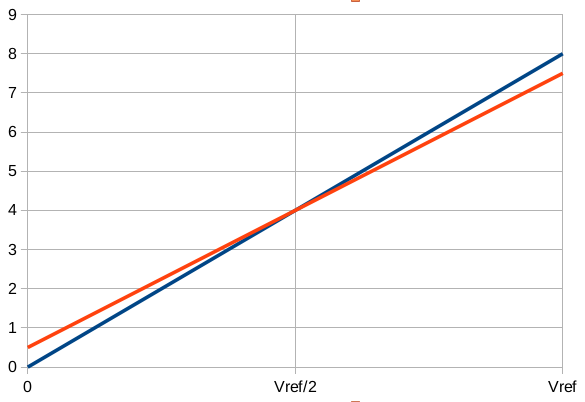
\includegraphics[scale=0.3]{figures/images/literature/ADC_Offset_Error.png}
    \caption{ADC ofszet hibája}
    \label{fig:ADC_Offset_Error}
\end{figure}

Másik jellegzetes hiba a nem linearitás, ennek jellemzője, hogy a mérési 
tartományon belül még az ofszet hibát is figyelembe véve nem azt az eredményt 
kapjuk, mint amit elvártunk amelyet nehezebb korrigálni szoftveresen, mivel amíg 
az ofszet hibát egyszerűen lehet korrigálni csupán a 0 és $V_{ref}$ feszültség szintek 
megmérésével, addig ezt a hibát sokkal nehezebb kiküszöbölni, mivel az ADC 
eredménye nem lineáris, így több ismert mérési pontot kell felvenni és a számítás 
is sokkal bonyolultabbá válik. Ezen kívül lehetnek kvantálási hibák is, amikor az 
ADC egy bizonyos értéket sosem ad eredménynek, hanem a nála egyel kisebb/nagyobb 
értéket. Ez nem okoz nagy gondot azoknál az ADC-nél ahol nagy a felbontás, viszont 
az alacsony felbontású eszközök esetén nagyobb hibát eredményez.

\subsection{Digitál Analóg Konverter}

A Digitál Analóg Konverter feladata, hogy a processzor által értelmezhető digitális
értékeket analóg jelekké konvertálja amik a külső perifériáknak szükségesek.
Gyakran használják ahol pontos analóg jeleket kell vezérelni, ilyen egy VGA jel
vagy zene lejátszása, viszont bármire felhasználhatóak ahol az egyszerű digitális
jelek nem elegendőek. Ebben a projektben az alkatrészek azonosítására és a 
karakterisztika diagram kirajzolására van felhasználva.

Működése hasonlóképpen működik, mind az Analóg Digitál Konverter-é, viszont fordítva.
Egyes DAC-eknek van belső referencia feszültségük, vagy kell külsőleg egyet alkalmazni.
Ez a jel lesz DAC maximális analóg kimenete amikor a digitális bemeneten a maximális
érték érkezik és 0V lesz a kimenete amikor 0 értékű digitális érték érkezik. Ideális
esetben e két pont között az átmenet lineáris, így minden köztes értékre egy lineáris
összefüggés alapján ki lehetne számolni [\ref{DACequation}], ahol D a digitális bemenet
ami 0 és $2^{res}$ között kell legyen.
\begin{equation}
    \label{DACequation}
    \begin{split}
        V_{out} &= V_{ref} \frac{D}{2^{res}}
    \end{split}
    \end{equation}

\section{Felhasznált eszközök}


\subsection{Raspberry pi pico}

Ez a teszter legfontosabb eleme [\ref{fig:Pico_pinout}], ez a vezéreli a teszter többi részét. A Raspberry 
által kifejlesztve, viszont nem, mint a többi termékük ezen nem fut egy operációs 
rendszer és használható, mint egy számítógép, hanem mint egy hagyományos 
mikrovezérlő. A mikrovezérlő magját egy Dual-core ARM Cortex M0+ processzor, 
aminek a frekvenciáját dinamikusan változtatható 16Mhz és akár 280Mhz közt. A 
memóriája is elegendő 264KB of SRAM a változók tárolására a program futása során 
és 2MB Flash memória a program kód tárolására. Lehetőség van csak RAM-ból futtatni 
is a kódot, ilyenkor nagyobb órajel is elérhető ami elérheti a 450Mhz-et is.

A vezérlő úgy van megtervezve, hogy THC (Through Hole Component) és SMT 
(Surface Mount Component) komponensként is lehet alkalmazni, 
ezt a castellated pinekel éri el, amelyeket lehet forrasztani közvetlen SMT 
komponensként és a pinek távolsága annyi, mint egy átlagos breadboard sortávja így 
egy male-male header forrasztásával breadboardon is alkalmazható. 

Hardveresen 
megtalálható 2xSPI, 2xI2C, 2xUART, 3x12-bit ADC, 16xszabályozható PWM csatorna és 
összesen 26 GPIO van kivezetve a felhasználó fele. Egy pin több dologra is képes 
ez az alábbi pinout diagramon is látható. Programozás során beállítható, hogy 
USB-t használja soros portként így egyszerűen használható egy számítógéppel való 
kommunikációra. Megtalálható 8 PIO (programable I/O) amivel hardveres protokollokat 
lehet létrehozni, ha valami egyedi kell egy különleges komponens vezérlésére. 


\begin{figure}[H]
    \centering
    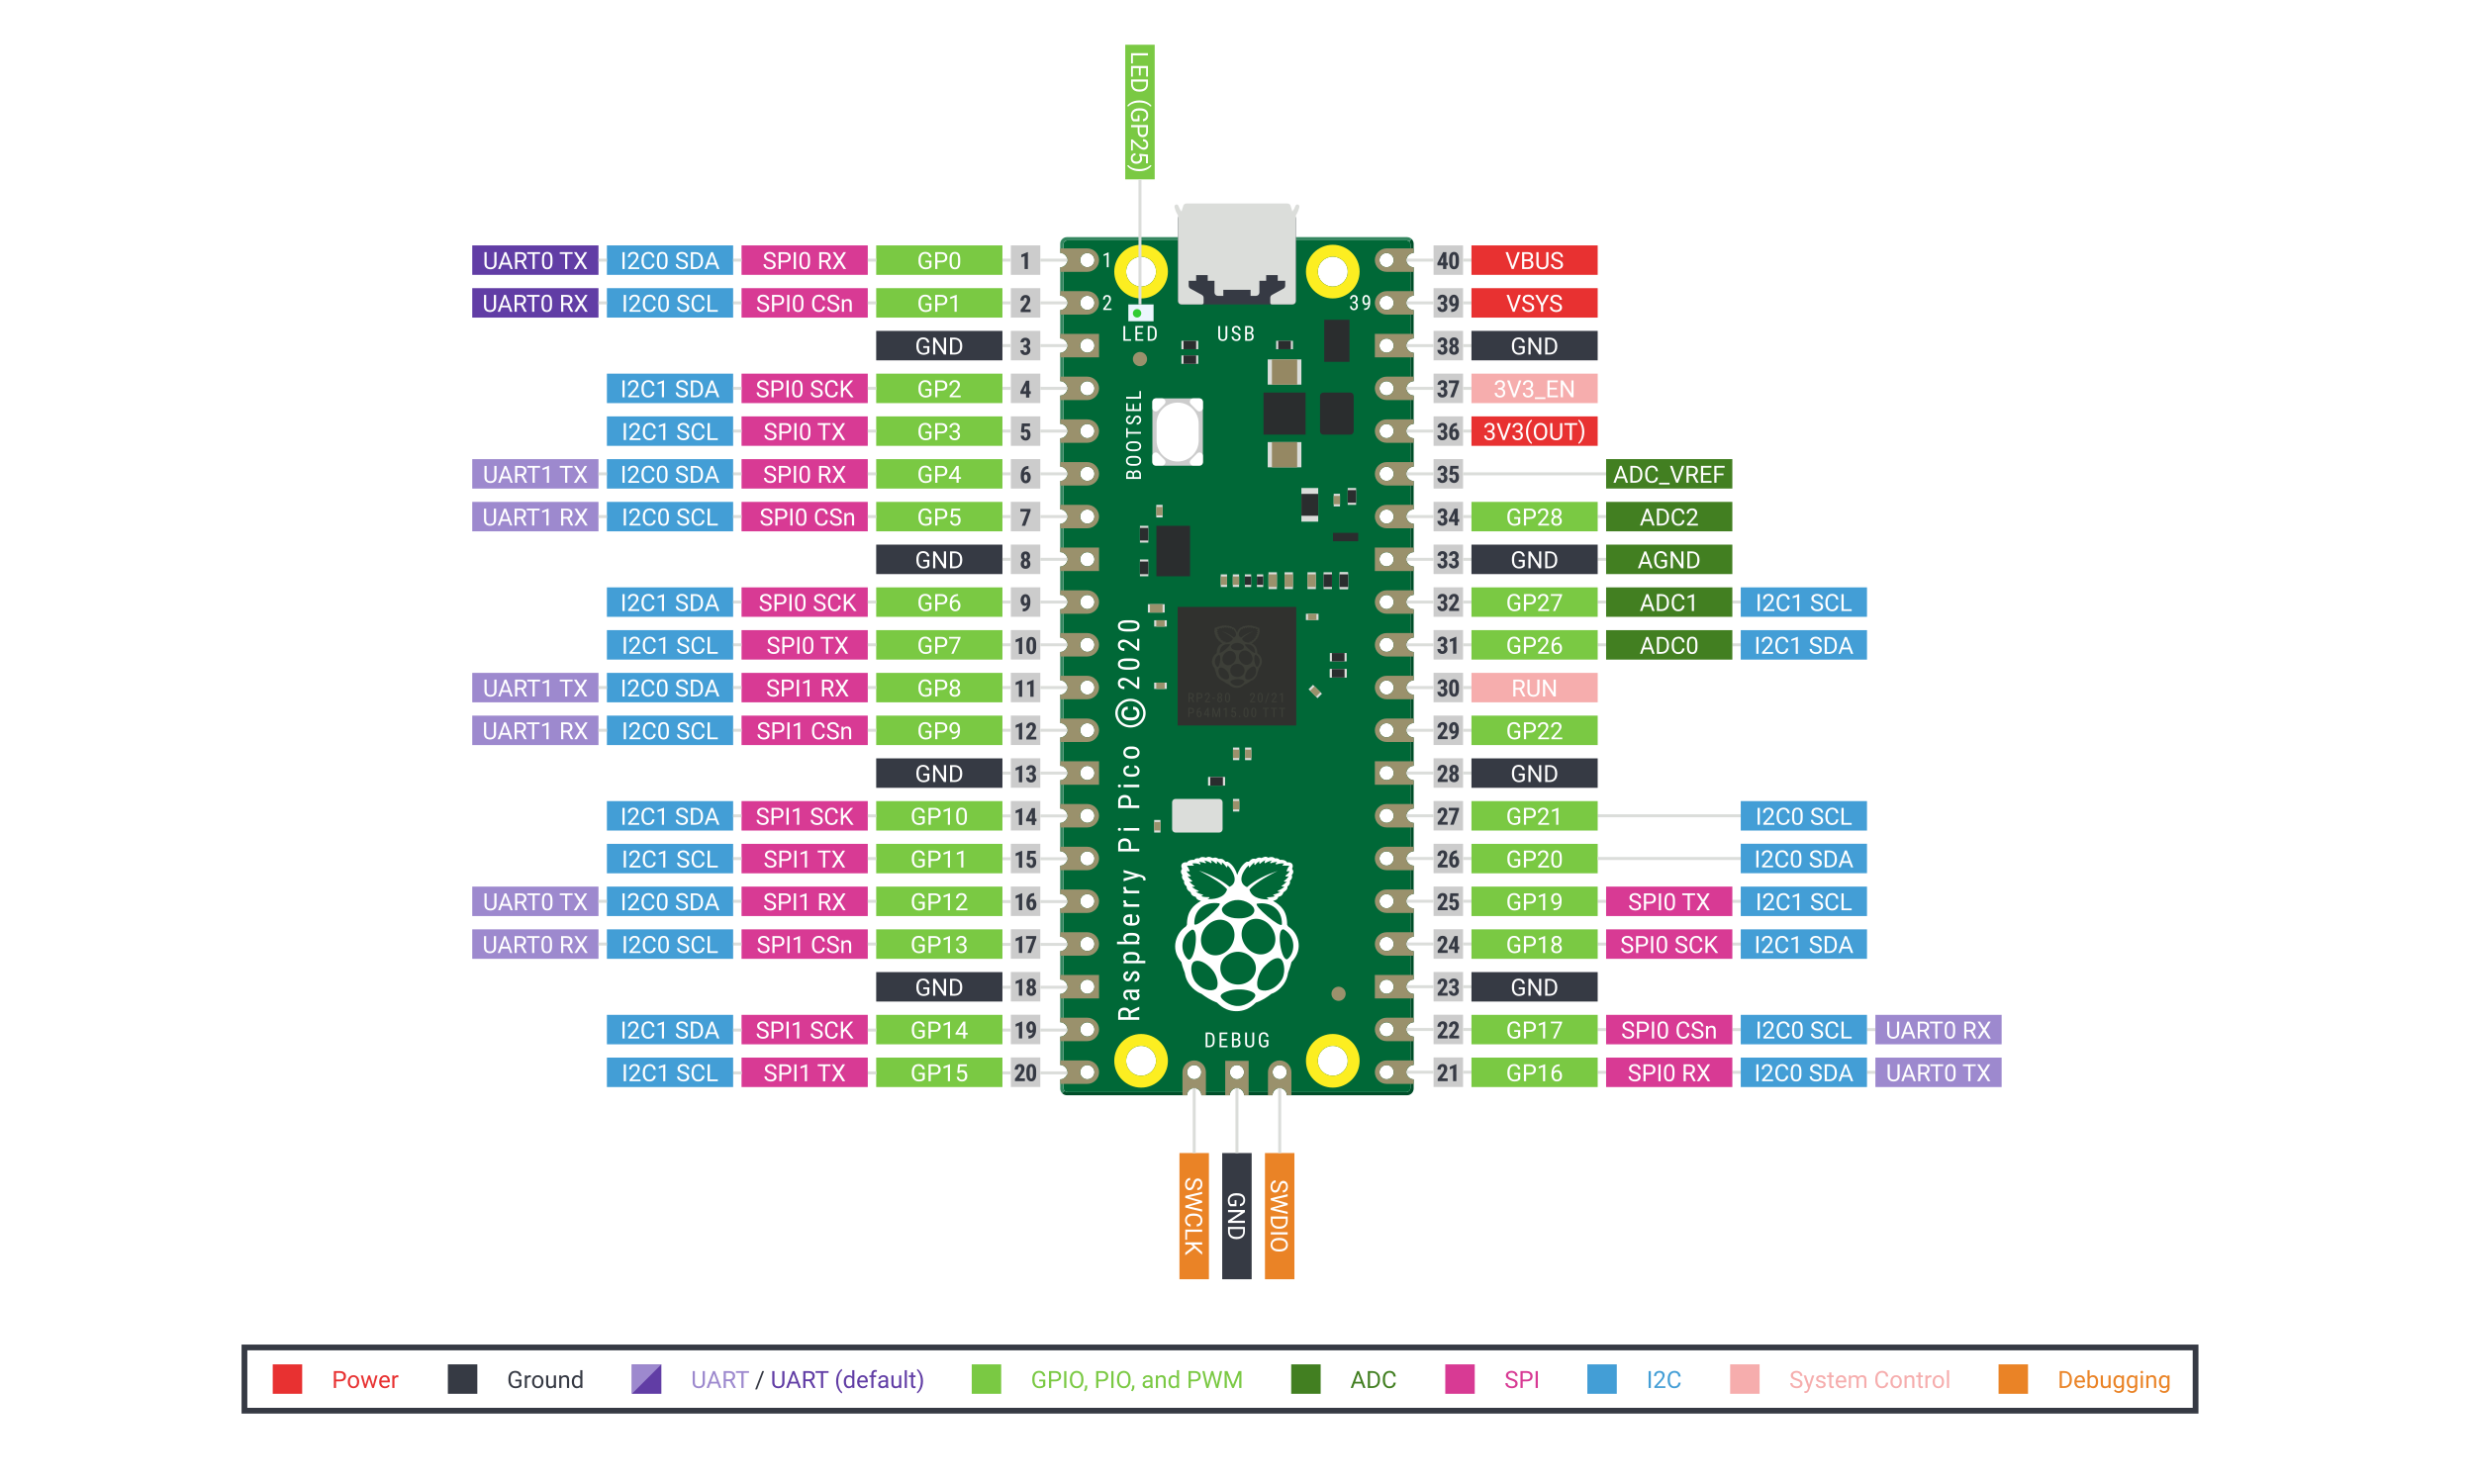
\includegraphics[scale=0.2]{images/literature/pico-pinout.png}
    \caption{Pico pinout}
    \label{fig:Pico_pinout}
\end{figure}


\subsection{ILI9341 kijelző}

Az adatok kijelzésére egy ILI9341 [\ref{fig:ILI9341 kijelző}] kijelzőt használtam.
Egy egyszerűbb kijelző is megfelelne a célra, akár csupán egy karaktereket megjelenítő
kijelző is elegendő lenne a célra, ha nem kellene a karakterisztika diagram. A 
célra megfelelne egy egyszerű OLED kijelző is. Viszont ez a kijelző már a rendelkezésre
állt a projekt tervezése előtt is, így fel lehetett használni a kijelzőt erre a 
projektre.

Ezen fognak megjelenni az mérés eredményei, mint a komponens értékei, a lábkiosztása
és a karakterisztika diagramja. A képernyő képes 16 bites színes kép megjelenítésére,
viszont ez nem fontos ennél a projektnél. Viszont a nagy 240*320 as felbontása és
a 2.2" kijelző mérete nagyban segít, hogy könnyen olvasható legyen. A kijelző rendelkezik
beépített háttérvilágítással is, így fényes helyen is jól látható.
A kijelző SPI protokollon keresztül kommunikál a mikrovezérlővel és rendkívül stabil,
akár 68Mhz-es órajellel is stabilan és megbízhatóan megkapja az adatokat a mikrovezérlőtől.
Ennek az eredménye a rendkívül gyors képernyő váltás, így a felhasználó nem kell
arra várjon, hogy az adatok megjelenjenek a kijelzőn.

Az adatok beírása pixel szinten történik amelyek a kijelző memóriájában elmentődnek, 
előre meg kell határozni, hogy milyen
zónában történik az írás és azután lehetséges csak az adat küldése és belsőleg automatikusan
a következő mezőt címzi meg, ahogy megérkezett az adat az előzőnek. Ennek az eredménye,
hogy írás során nem kell figyelembe tartani a kijelző belső memória címét, csak az 
adat sorrendjét. Ez egyszerűsíti a programozó dolgát és csökkenti a küldési
időt.

\begin{figure}[H]
    \centering
    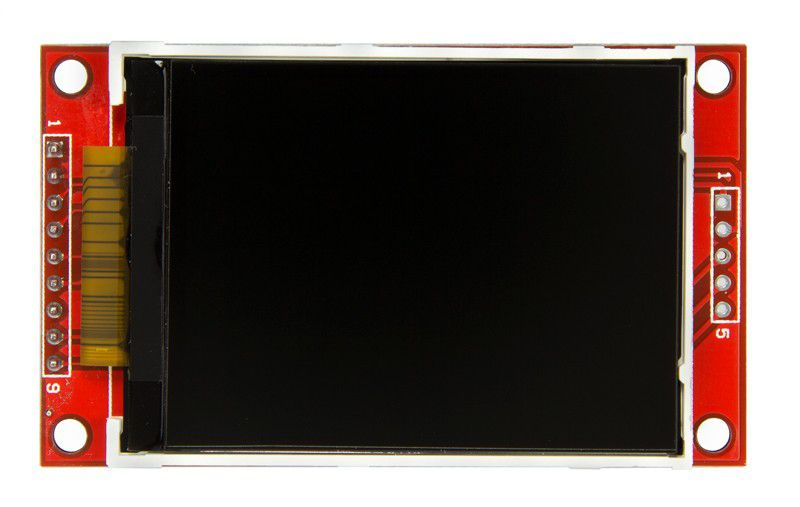
\includegraphics[scale=0.5]{images/literature/ILI9341.png}
    \caption{ILI9341 kijelző}
    \label{fig:ILI9341 kijelző}
\end{figure}

\subsection{Digitál Analóg Konverter}

Az analóg jelek generálására egy DAC8565IAPWR [\cite{DAC}] van alkalmazva, 
amelynek felbontása 16 bit.
Ennek 4 egymástól független kimenete van, amelyek belsőleg pufferelve vannak,
így terhelés esetén sem változik. 

A DAC-nak van egy belső 2.5V-os feszültség referenciája,
viszont ez külsőleg felülírható egy külső feszültség referenciával. Ebben az 
esetben szükség volt erre, mivel a teljes ADC mérési tartományra szükség van
ami 3.3V. Ez egy egyszerű 3.3V-os feszültség referenciával lett elérve, viszont
ebben az eseten egy parancsot kell küldeni a DAC-nak, hogy a külső referenciát használja,
mivel nem áll át automatikusan, rövid időre nem gond, hogy mindkettő aktív, viszont
nem ajánlott huzamosabb ideig ilyen helyzetben tartani.

A DAC SPI protokollt használ amiből 8 bit a parancs bit és 16 bit az adat.
Lehetőség van az adatok azonnali betöltésére és a kimenet változtatására, és
arra is van lehetőség, hogy csak az adatot elmentse és egyszerre frissítse az
összes kimenetet. Erre lehetőség van szoftveresen is, amit az SPI parancs
részében lehet kódolni, ebben a projekt esetében is ez van alkalmazva. 

\subsection{Analóg kapcsoló}

Mindegyik analóg jelet egyszerre 1 ellenálláson keresztül rá kell kapcsolni a komponensre,
viszont az ellenállás váltható kell legyen mérés közben, nagy sebességgel, így a manuális
kapcsolás nem lehetséges. Erre a célra egy analóg kapcsoló van alkalmazva amely egy közös
bemenetet 3 különböző kimenetre képes kapcsolni, melyeken az ellenállások találhatóak.
A kimenet kiválasztása nem használ kommunikációs protokollt, csak a "IN" portokra érkező
digitális jelek segítségével történik. Minden esetben maximálisan 1 kimenet aktív a többi
a nyílt áramkörben van és arra is van lehetőség, hogy a bemenet 1 kimenetre 
se legyen kapcsolva. A kimenet kiválasztása a következő táblázattal lehetséges.
[\ref{fig:ASwitchFuntionTable}]

\begin{figure}[h]
    \centering
    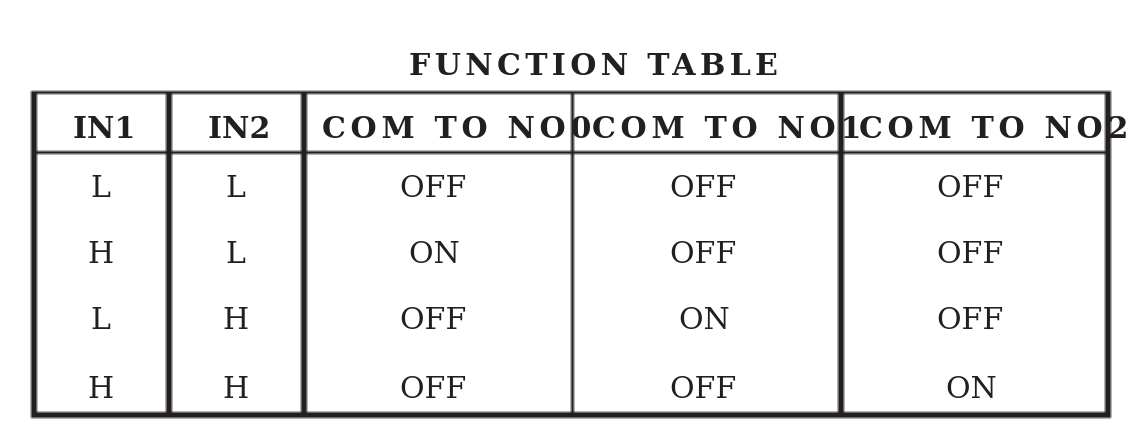
\includegraphics[scale=0.3]{images/literature/ASwitchFunctionTable.png}
    \caption{Analóg kapcsoló funkcionális táblázata}
    \label{fig:ASwitchFuntionTable}
\end{figure}



\section{Felhasznált Technológiák}

\subsection{A programozási nyelv}

A mikrovezérlő programozásához a C++ nyelv van használva. A mikrovezérlő alkalmazni 
tudja a standard könyvtárakat, és az objektum orientáltságából fakadóan lehet az 
OOP sémákat alkalmazni, amellyel bonyolultabb feladatokat is meg lehet valósítani
már megoldott példák alapján, ezzel lecsökkentve a programozási időt.
Mivel a standard C++ legtöbb függvényét ezért a kód hasonló, mintha az egy számítógépre
lett volna írva, csupán az alacsony szinten kell egyedi függvényeket meghívni.
Ezek a függvények jól dokumentáltak és a legtöbb esetben van egy teljesen működőképes
példa program.

A mikrovezérlő csak C/C++ és micropython nyelveken programozható, viszont ennek
kevesebb a dokumentációja és lassabb, így nem alkalmas erre a feladatra.


\subsection{Mikrovezérlő felprogramozása}

A projekt lefordítására szükséges egy egyedi compiler, ami a programot lefordítsa
a mikrovezérlő által megérthető nyelvre. Ez telepíthető a Raspberry oldalán megadott 
utasításokkal, viszont ez lehetséges, hogy frissül, így telepítés előtt ajánlott
azt követni. A compiler Linux és Windows rendszereken is használható. A fordítás után
generál egy .uf2 fájlt, ezt kell feltölteni a mikrovezérlőre amit elment a Flash
memóriájában és automatikusan indul amit bekapcsol.

A programozásra csak egy micro-USB kábel szükséges. A számítógéphez csatlakoztatás előtt
a mikrovezérlőn található BOOTSEL gombot lenyomva kell tartani és így csatlakoztatni a
számítógéphez, ekkor megjelenik mint egy külső tároló. Ebbe a tárolóba fel kell másolni
a generált .uf2 fájlt, amint ez megtörtént lecsatlakozik és futtatni kezdi a programot.


\subsection{SPI}

A kommunikációs protokoll amit a kijelző és a DAC használ. A mikrovezérlőnek vannak
beépített függvényei és specifikus pinei amellyel képes hardver szinten kommunikálni
külső eszközökkel. Ez egy full duplex protokoll, vagyis képes egyszerre mindkét eszköz
adatot küldeni, anélkül, hogy egymást zavarnák. Ez 2 külön vezetéken
keresztül történik, órajel szinkronizációval.

Az SPI egy mester szolga alapú protokoll, általános esetben 1 mester van (pl. egy 
vezérlő), de lehet több mester is, amennyiben csak 1 mester aktív és a többi mester
a kimeneteit magas impedanciára kell helyezze (High Z), hogy ne befolyásolja az 
adatok küldését. 


A szolgák száma bármennyi lehet, viszont nem szokott nagyszámú lenni, mivel minden
szolgának egy külön vezeték kell az aktiválásra, ez a CS (chip select), amely 
legtöbb esetben aktív és csak akkor lehet a bizonyos eszközzel kommunikálni, amennyiben
ez első lépésben megtörtént.

Az SPI egy órajellel szinkronizált protokoll, az órajelet a mester szolgáltatja,
amely nincs standardizálva, csupán az eszköz maximális órajellel frekvenciája 
alatt kell legyen. Az eszközöktől függően nyugalmi helyzetben az órajel lehet alacsony
vagy magas szinten.

Az adatok küldésére 2 vezeték szükséges, ezek a MOJSI (master out slave in), ezen a
vezetéken érkezik az adat a mester felől a szolga felé. Az adatok kiolvasása nincs
standardizálva, így az eszköztől függően az adatot olvashatja az órajel felfutó vagy a 
lefutó élén. Az adat a mester felé a MISO (master in slave out) vezetéken érkezik,
viszont a mester kell órajelet generáljon, hogy a szolga el tudja küldeni az adatokat.

\section{A rendszer Blokk váza}

Az alábbi árbán [\ref{fig:blockDiagramm}] látható a rendszer blokk Diagramja, a fő vezérlő jelekkel.
A rendszer 2 SPI perifériával kommunikál, ezek a kijelző és a DAC, az analóg kapcsoló vezérlő jelei 
egyszerű digitális jelek, mint ahogyan a LED vezérlő jelei. A teszter socket mindhárom lába egy-egy ADC
csatornához van csatlakoztatva, ezen méri a mikrovezérlő a tesztelés során a feszültség szinteket.
A kapcsoló a RUN bemenetre van kapcsolva, ez engedélyezi a mikrovezérlő futását amíg feszültség érték 
található rajta vagy nincs bekötve. Amennyiben ez földre kerül akkor a mikrovezérlő leáll és restellődik.

A rendszerhez működéséhez szükséges egy 5V-os feszültség forrás, ez lehet egy általános USB
tápforrás, vagy lehetséges direkt 5V csatlakoztatása is. Az áramerősség alacsony, így nem közelíti
meg az 500mA-es áramerősség határt amit egy átlagos USB képes leadni. Külső akkumulátorról
is táplálható. Amennyiben egy számítógéphez, vagy egy olyan eszközhöz van csatolva ami képes 
a serial portot olvasni akkor a mérési eredményeket automatikusan elküldi azon keresztül a 
másik eszköz felé. 


\begin{figure}[h]
    \centering
    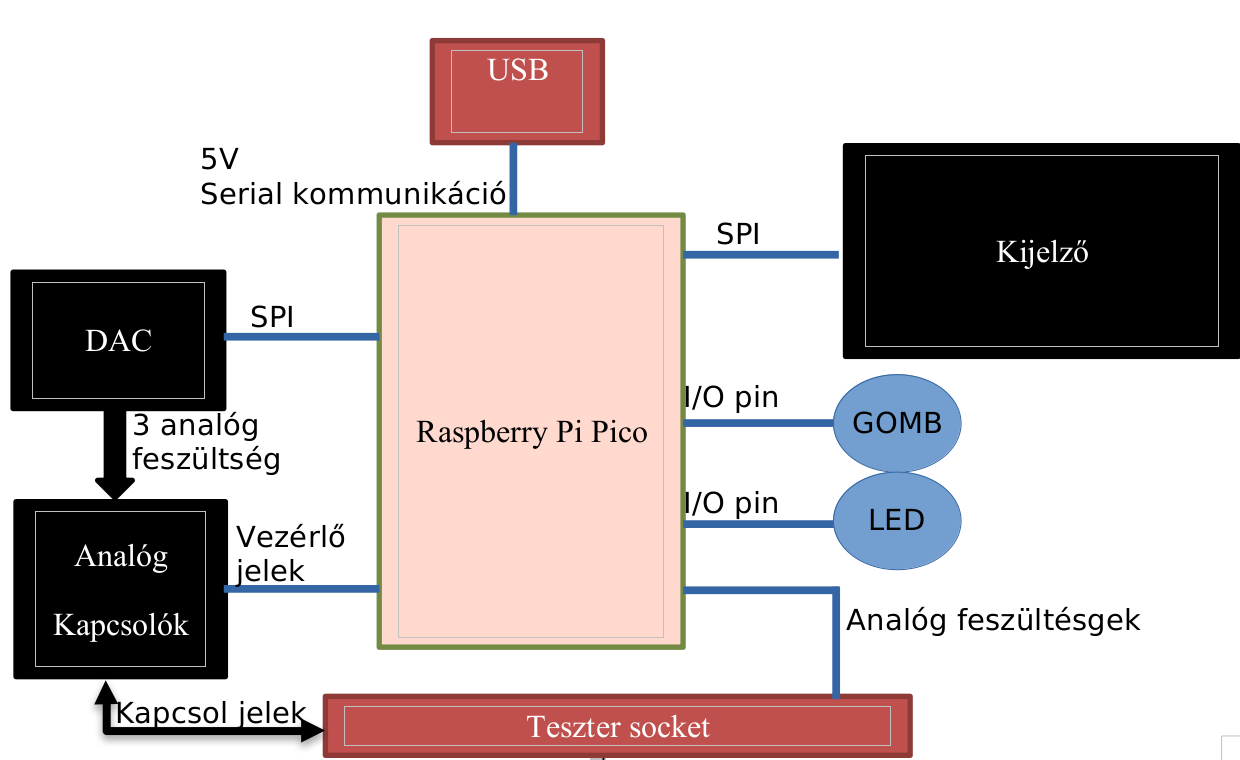
\includegraphics[scale=0.3]{images/literature/blockDiagramm.png}
    \caption{A rendszer blokk váza}
    \label{fig:blockDiagramm}
\end{figure}


\section{Hasonló eszközök}

Egy hasonló rendszer már megvalósult [\cite{similarSystem}] ami egy Arduino 
[\cite{ArduinoAtmega}] 
mikroprocesszoron alapul. Ez egy egyszerűbb rendszer, ami csupán ellenállásokat használ az 
alkatrészek felismerésére és egy kijelzőt az adatok megjelenítésére. Ebből több fejlesztés is 
kialakult, több minden tesztelésére és nagyobb pontosság elérésére, miközben a rendszer 
egyszerűségét fenntartani. Ezek a rendszerek viszont nem használnak DAC-ot és ezért nem képesek 
karakterisztika diagramot készíteni. Ezen kívül nem csatlakoztatható egyszerűen számítógéphez, 
csupán újraprogramozás céljából, így minden esetben kell tartalmazzanak egy kijelzőt, ami 
növeli a költségeket. Az általános működésük hasonló, mint ebben a projektben, viszont itt 
precízen lehet változtatni a feszültséget, nem csak kapcsolni földre vagy tápfeszültségre.
Az bekötése hasonlóképpen történik: lásd [\ref{fig:basicTesterConnection}]

\begin{figure}[h]
    \centering
    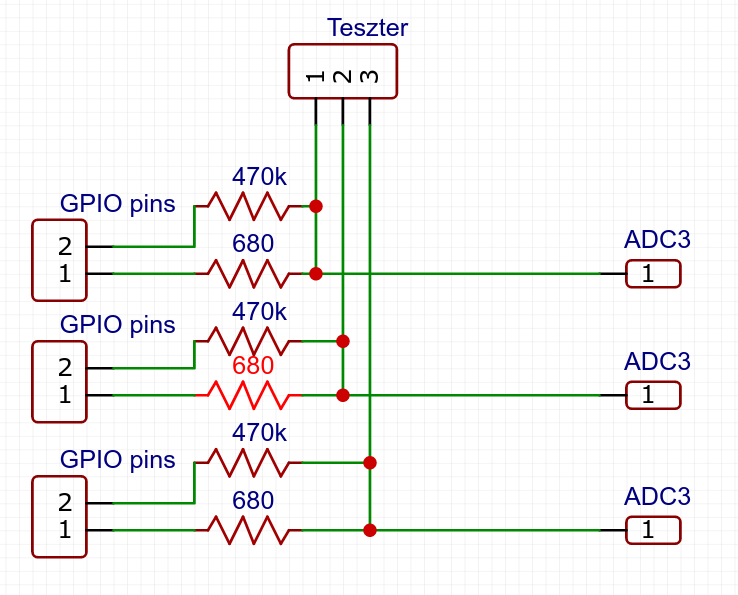
\includegraphics[scale=0.3]{images/literature/OrgTesterConnection.png}
    \caption{Eredeti teszter bekötési rajza}
    \label{fig:basicTesterConnection}
\end{figure}

Mindegyik GPIO pin lehet csatolva földre, vagy tápfeszültségre, de le is lehet kapcsolva, így 
nem befolyásolja az áramkör működését. Az ADC pin meg lehet ADC üzemmódban, ilyenkor nem befolyásolja
az áramkört, viszont lehet földre, vagy tápfeszültségre is kapcsolni, ilyen esetben port ellenállás
nélkül csatolódik az áramkörre.

Viszont szintén hordozható egy 9V-os elem segítségével és az eredmények megjelennek egy
kis LCD kijelzőn, ebből több verzió is létezik, van amely csak egy karakter kijelzőt
használ, van amelyik egy színes kép kirajzolására is alkalmas kijelzőt alkalmaz. 

A tesztelés néhány másodpercbe telik, nagy méretű kondenzátorok esetén telhet több időbe,
viszont ebben az esetben csak annyi idő, míg a legkisebb ellenálláson keresztül képes feltölteni
a kondenzátort.

\chapter{Rendszer specifikációja és architektúrája}
\section{Rendszer Követelmények}

\subsection{Funkcionális követelmények}

A rendszer elvár egy 2 vagy 3 lábbal renddelkező alkatsész csatlakoztatását a 
teszter sockethez, olyan módon, hogy elektronikusan is csatolva legyen. 
Az alkatrész lehet ellenállás, kondenzátok, dióda vagy tranzisztor, viszont a 
rendszer csak maximális feszültsége 3.3V, így amennyiben nagyobb nyitó
feszültség szükséges az alkatrésznel akkor abban az esetben nem képes
detektálni azt.

A rendszer fő követelménye a tesztelés leegyszerősítése, így egy átlagos,
elektronikai imeretekkel nem rendelkező felhasználó is egy rövid 2 perces 
bemutató után is magabiztosan tudja használni. Ezt a felháló által élérhető
bemenetek csökkentésével lett elérve, mivel a felhasználó könnyebben 
tud egy olyan eszközt használni ahol a bemenetek száma minimális.

A tesztelés az indulástól kezdve automatikus, így tesztelés során a felhasználó
nem kell semmit se tegyen, a tesztelés vége a 2 jelző LED felkapcsolósóval van
jelezve és az eredmények a rendszeren megtalálható kijelzőn jelennek meg és 
amennyiben a rendszer egy számítógéphez van csatolva abban az esetben 
a Serial porton keresztül itt is megjelennek az eredmények.

\subsection{Nem funkcionális követelmények}

A rendszer lehetőleg nagy gyorsaságú legyen, mivel ha sok időt venne igénybe
a mérés akkor abban az esetben gyorsabb lenne leolvasni az alkatrész azonosítóját
és az interneten rákeresni, vagy kézzel lemérni egy multiméter segítségével.
A mérés átlagosan 3 másodperc alatt el kell végezzen egy teljes azonosítást. 
Ez a legtöbb esetben rövidebb idő, csupán
a nagy méretű kondenzátorok esetében lehetséges ennek túllépése.

A rendszer egyedülálló módon is alkalmazható akár egy külső 
akkumulátorról is táplálva, így nincs operációs rendszer követelménye
az alapszintű működéshez.

Hordozhatóség is elengedhetetlen, hogy könnyedén mindig kéznél legyen.
Ezért esett a választás az USB-n keresztül való táplálásra, mivel ez 
manapság sokkal elterjedtebb, mint az eredeti tranzisztor teszter ami egy
9V-os elemet használ ami kevésbé gyakori és elem lévén le tud merülni, pont 
akkor amikor a legjobban kellene.

A rendszer tervezésekor, mivel ez egy mikrovezérlőn fut így a 
tárhely és memória limitált. Amiből a legfontosabb a memória, ebből 
csupán 264KB található, így figyelembe kellett ezt tartani. Itt 
legfőképpen a kijelzőn volt szükség az optimalizációra, mivel 
lehetséges lett volna, hogy a nagy része csak a kijelzővel lett volna elfoglalva.

A mérés során a pontosság nem a legfőbb kritérium, viszont egy megközelítő
értéket kell adjon. Az értékek +-10 százalékban eltérhetnek a valós értéktől, 
ami még mindig elégséges az azonosításra. 

A projekt verziókövető rendszer jelenlét mellett készült, amivel
vissza lehetett állítani esetlegesen elrontott fájlokat működő állapotába
és egy biztonsági másolatkéni is szolgált.

\section{A rendszer Blokk váza}

Az alábbi árbán [\ref{fig:blockDiagramm}] látható a rendszer blokk Diagramja, a fő vezérlő jelekkel.
A rendszer 2 SPI perifériával kommunikál, ezek a kijelző és a DAC, az analóg kapcsoló vezérlő jelei 
egyszerű digitális jelek, mint ahogyan a LED vezérlő jelei. A teszter socket mindhárom lába egy-egy ADC
csatornához van csatlakoztatva, ezen méri a mikrovezérlő a tesztelés során a feszültség szinteket.
A kapcsoló a RUN bemenetre van kapcsolva, ez engedélyezi a mikrovezérlő futását amíg feszültség érték 
található rajta vagy nincs bekötve. Amennyiben ez földre kerül akkor a mikrovezérlő leáll és restellődik.

A rendszerhez működéséhez szükséges egy 5V-os feszültség forrás, ez lehet egy általános USB
tápforrás, vagy lehetséges direkt 5V csatlakoztatása is. Az áramerősség alacsony, így nem közelíti
meg az 500mA-es áramerősség határt amit egy átlagos USB képes leadni. Külső akkumulátorról
is táplálható. Amennyiben egy számítógéphez, vagy egy olyan eszközhöz van csatolva ami képes 
a serial portot olvasni akkor a mérési eredményeket automatikusan elküldi azon keresztül a 
másik eszköz felé. 


\begin{figure}[h]
    \centering
    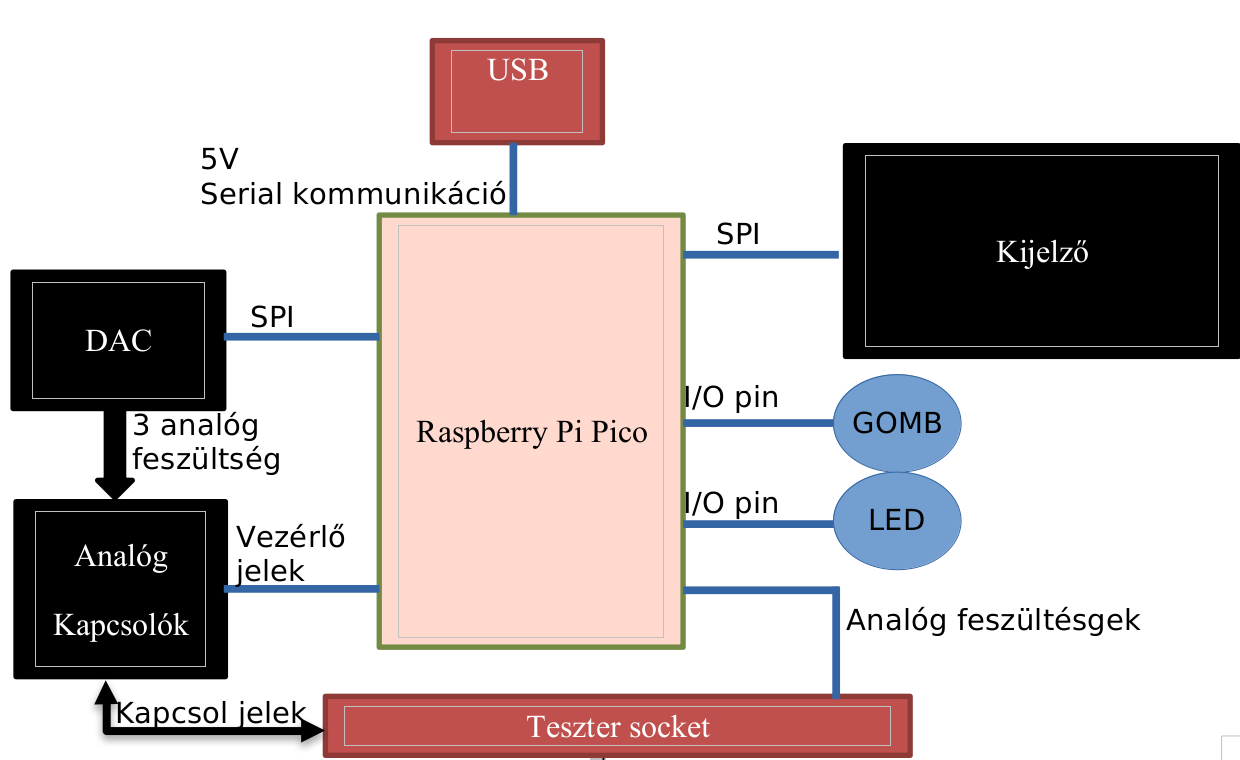
\includegraphics[scale=0.3]{images/literature/blockDiagramm.png}
    \caption{A rendszer blokk váza}
    \label{fig:blockDiagramm}
\end{figure}

\section{A rendszer osztály diagrammjai}

\subsection{Kijelző vezérlő}

Az alábbi ábrán[\ref{fig:displayClassDiagram}] a kijelző vezérlésért felelős osztályok láthatóak.
Ez a rendszer többi részétől elszigetelt rész, amely csupán 
megkapja az eredményeket a mérések után és megjeleníti azt.


\begin{figure}[h]
    \centering
    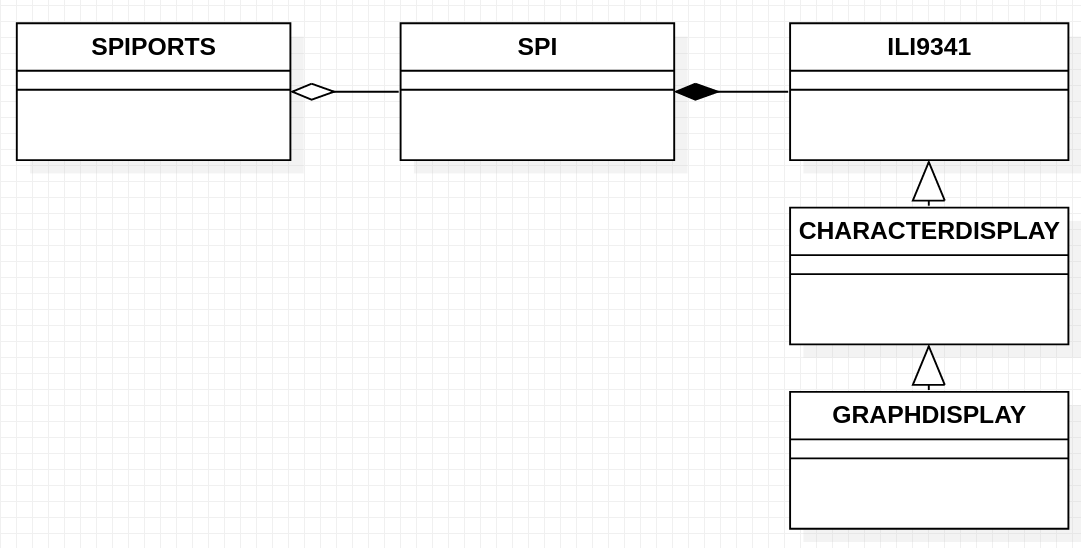
\includegraphics[scale=0.4]{images/diagrams/displayClassDiagram.png}
    \caption{A kijelző osztály diagramja}
    \label{fig:displayClassDiagram}
\end{figure}

Az ILI9341 osztály az alapszintű vezérlésért felelős, itt csak az 
adat küldési funkcionalitás és a képernyő inicializásása van
implementálva. A CHARACTERDISPLAY osztály kibővíti ezt és lehetővé
teszi egyszerű szöveg megjelenítését a kijelzőn.
A GRAPHDISPLAY kibővítve ezt képes megjeleníteni grafikont
a kijelzőre beépített skálázással, hogy lehetőleg az egész kijelzőt kihasznélja.


\subsection{Mérő áramkör osztály diagrammja}

Alábbiakban [\ref{fig:ControlClassDiagram}] a rendszer az adatok méréséért felelős osztályai láthatóak,
ezek az osztályok alkotják a mérő eszközök vezérlését, mint a 
DAC és az analóg kapcsolók és az adatok mérését.
A rendszrben az ADC globális osztály és abból csak egy van.

\begin{figure}[H]
    \centering
    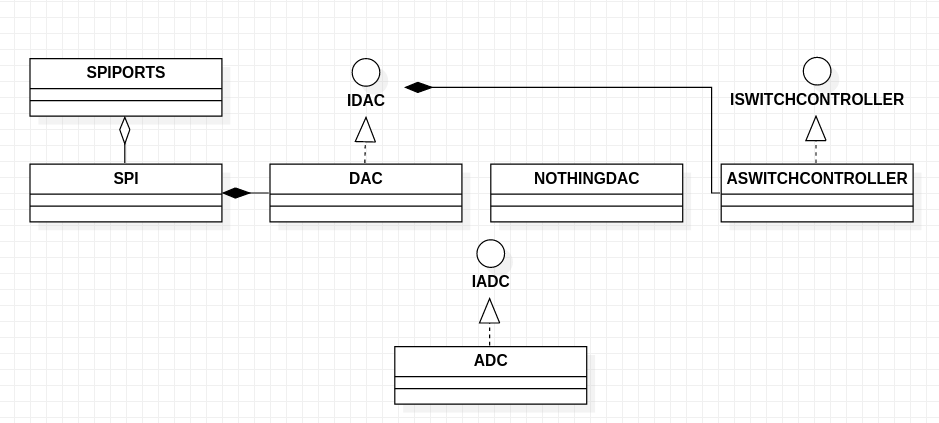
\includegraphics[scale=0.5]{images/diagrams/ControlClassDiagram.png}
    \caption{A vezérlő osztályok diagramja}
    \label{fig:ControlClassDiagram}
\end{figure}


\subsection{Számításokért felelő osztályok}

A következő osztályok[\ref{fig:CalculateClassDiagram}] felelnek a részeredmények kiszámításáért. A 
számításokat az ACALCULATE osztály végzi, az ADCCORRECTER osztály
feladata az ADC konstans hibájának a kiküszöbölésére. Az 
ISWITCHCONTROLLER az előző [\ref{fig:ControlClassDiagram}] ábrán látható
vezérlő rendszerrel van kapcsolatban. A BASEVALUES osztály a mérés során
történt ideiglenes adatok tárolására szolgál.


\begin{figure}[H]
    \centering
    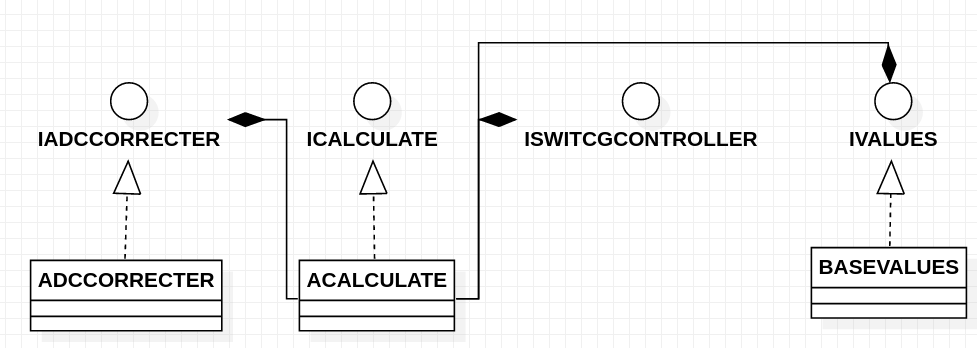
\includegraphics[scale=0.4]{images/diagrams/CalculateCalssDiagram.png}
    \caption{A számításokat elvégző osztályok diagramja}
    \label{fig:CalculateClassDiagram}
\end{figure}

\section{A mérés folyamat ábrája}

A mérés lépései a következőképpen történik[\ref{fig:CalculateStateDiagram}].
Első lépésben ellenállásra tesztel, ez ha nem talál semmit,
vagyis egyik teszter láb sincs csatlakoztatva, vagy nem reagál akkor 
a tesztelt komponens hibás, vagy nincs csatolva. Amennyiben valamilyen 
eszköz érzékelve van abban az esetben megpróbálja megmérni az ellenállás 
értékét, miközben figyelve arra, hogy ellenőrizzen lehetséges diódára is.
Ezt úgy oldja meg, hogy a dióda ellenállástól eltérően csak egy irányban vezet és
a feszültség esés konstans az áramerősségtől független.

Amennyiben dióda van detektálva abban az esetben a dióda útvonalon folyatódik a
tesztelés, különben megpróbálja megmérni az alkatrész kapacitását.

A dióda esetben ellenőrzi, hogy az alkatrész az 2 inverz dióda, és 
megméri a nyitó feszültségét. Amennyiben nem 2 inverz dióda, akkor abban az esetben
teszteli tranzisztorra is, ebben az lépésben képes az NPN és PNP tranzisztorokat
is detektálni és meghatározza a tranzisztor lábkiosztását.

\begin{figure}[H]
    \centering
    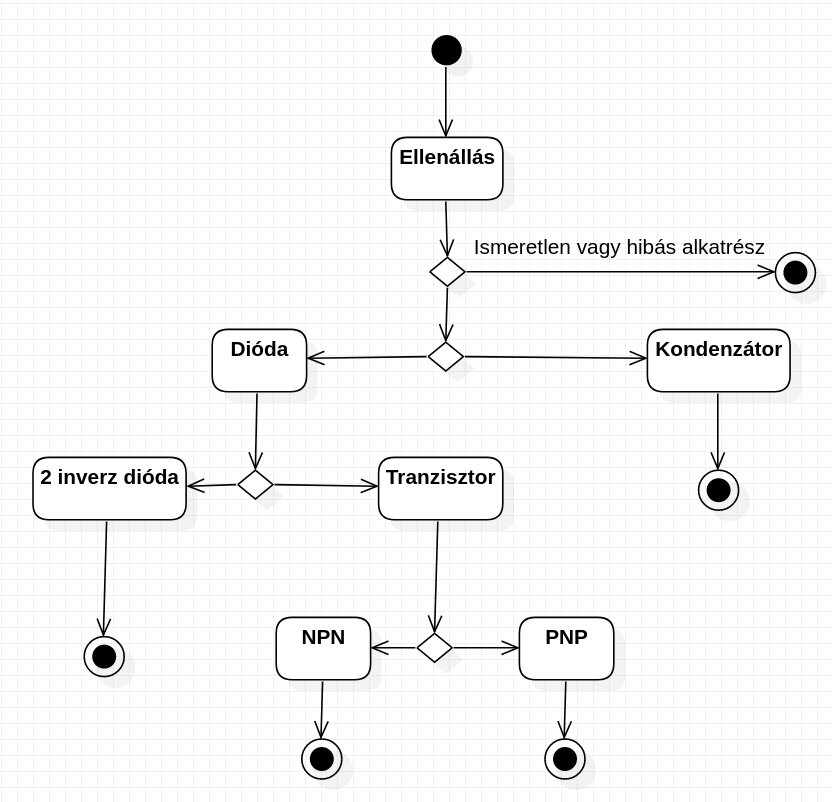
\includegraphics[scale=0.55]{images/diagrams/stateDiagram.png}
    \caption{A mérés fázisai}
    \label{fig:CalculateStateDiagram}
\end{figure}

%--------------------------------------------------------------------

\section{Mérő áramkör}

A rendszer hasonlóan épül fel, mint a példaként használt rendszer \cite{similarSystem}, viszont néhány módosítással.
Viszont az elméleti alapja hasonló. A komponens lábára egy ellenálláson keresztül feszültséget kapcsolva és a 
feszültség mérésével az ellenállás után meg lehet állapítani az áramerősséget és a feszültség esést a komponensen.
Ezekből az értékekből számítások segítségével ki lehet számolni, hogy mi az ismeretlen komponens (ennek a leírása
és lépései a későbbiekben lesznek részletezve) és értékét. A jelenlegi rendszer mérő áramkör része a következőkben
látható. [\ref{fig:ownTesterConnection}]

\begin{figure}[H]
    \centering
    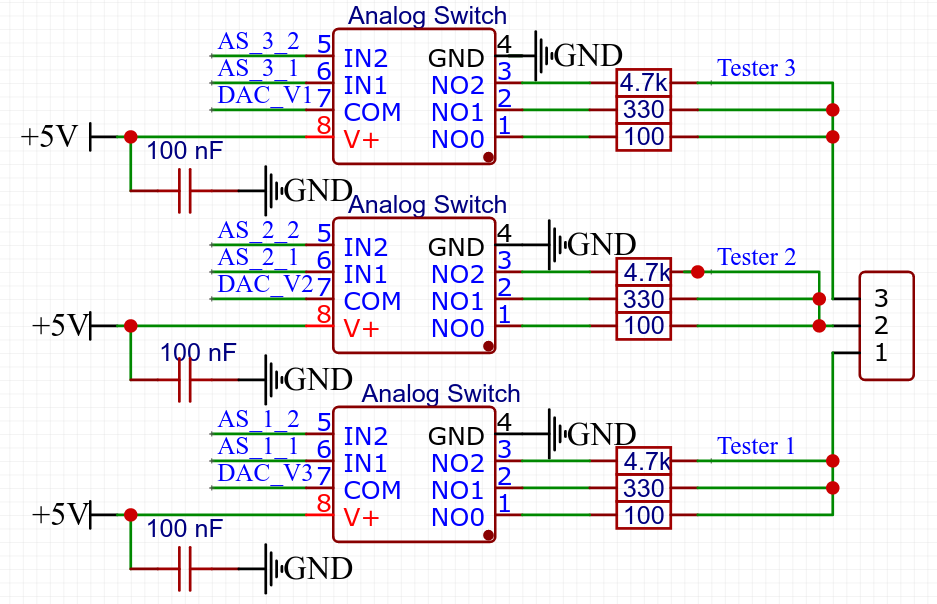
\includegraphics[scale=0.3]{figures/images/literature/TeszterConnections.png}
    \caption{Saját teszter bekötési rajza}
    \label{fig:ownTesterConnection}
\end{figure}

Ebben az esetben szükséges analóg kapcsolók használata, mivel az eredeti
teszter csak digitális jeleket használ amit direkt a GPIO-ról voltak kivezetve,
így az ellenállások közti váltásokért belsőleg a mikrovezérlő felt. Viszont ebben
az esetben a jelek analóg jellek amit egy külső DAC generál, így a mikrovezérlő nem
képes belsőleg kapcsolni ezeket ezért egy 3 kimenetes analóg kapcsoló van alaklmazva
erre a célra.

Mivel csak egy kapcsolón csak egy kimenet aktív egy időben, így az ellenállások után
a vezetékez összekapcsolhatóak, mivel azok nem fogják befolyásolni a rendszer működését,
erre a részre van kapcsolva az ADC egyik csatornája is, mivel itt a feszültség érték
azonos a komponens lábán található feszültséggel, így a komponenst nem kell módosítani,
hogy a feszültség látható legyen a lábán.

Az analóg jel 0V-3.3V közt lehetséges és a DAC maximálisan 50mA-t képes leadni, viszont
mivel a kondenzátorokat ki kell sütni csatlakoztatás előtt és külső tápfeszültség nem 
kapcsolható így a maximális áramerősség 33mA-nél nem lehet nagyobb semmilyen esetben.

A rendszer átlagolva nézi a feszültséget a komponens lábán, mellyel nagyobb pontosság
érhető el, mivel a zajok kevésbé befolyásolják a jelet. Viszont képes időben is mérni
a feszültséget, hogy hogyan változik a feszültség ahogy telik az idő. Az ADC 500.000 mérést
tud végezni másodpercenként, viszont ez lelassítható egy belső késleltetővel. Ami segítségével
a lassan változó jelek is megfigyelhetőek, mint például egy nagy kondenzátor töltödése.

\section{A mérés menete a felhasználó által}

Az PCB-n található felhasználó által használható eszközök egy kapcsoló és a 
teszter socket ahová a komponenst kell helyezni. A kapcsoló egy kétállású
kapcsoló mely a mikrovezérlőt leállítja, vagy elindítja ami által a mérés
automatikusan elindul.

A rendszer tartalmaz 2 LED-et ami a látható a következő fényképen is az
áramkörről is a kijelző jobb felső sarka fölött [\ref{fig:Aramkor}]. 
Amennyiben egyik LED sem világít, és a kijelző sem egy fehér hátteret
mutat abban az esetben a mikrovezérlő nem kap áramot, ilyenkor ellenőrizni
kell az USB kábelt.

Amennyiben a kijelző egy fehér képet mutat, viszont egyik LED sem világít akkor
a vezérlő reset állapotban van, ezt a vezérlő alatt levő kapcsoló ON 
pozícióba való állításával lehet orvosolni.

A mérés kezdetekor a piros LED felkapcsol, majd mérés befelyeztekor a Zöld 
LED is felkapcsol, ebben az esetben a mérés sikeres volt és az eredmény meg 
kell jelenjen a kijelzőn és az USB-n keresztül elküldve a számítógéphez.

A teszter sockethez nem lehet tápforrást vagy elemet csatlakoztatni, ide tartoznak
a nagy méretű kondenzátorok is, a kis méretűeket képes kisütni, de ajánlott 
csatlakoztatás előtt kisütni ezeket is.



\chapter{Részletes tervezés}
\section{Szoftver vezérlő rész}

\subsection{A beépített ADC használata}

A mikorvezérlőbe egy 3 csatornás ADC van beépítve, viszont egyszerre csak 1 
csatornát lehet olvasni, olvasás előtt át kell váltani arra a csatornára, amelyről
az adatot olvasni akarjuk. Az ADC hardver szinten egy 48Mhz-es órajelet kap és
egy mérés minimum 96 ciklusba telik, így 500k mérést végez másodpercenként, 
ezt viszont növelhető dinamikusan szoftveresen, így csökkenthető a mérési gyorsaság.


Az ADC képes DMA-n (direct memory access) [\cite{DMA}] keresztül kommunikálni a 
memóriával, így inicializálás után automatikusan elvégzi a méréseket az adott
csatornán. A csatorna inicializálása a következőképpen alakul. A méréseket
egy előre lefoglalt tömbbe teszi ami jelen esetben a \textbf{capture$\_$buf} tömb,
aminek a mérete \textbf{CAPTURE$\_$DEPTH} . A mérés után a tömbben időrendi sorrendben
kiolvashatók a mérések.


\begin{lstlisting}

    //ezeket csak egyszer a konstruktorban kell meghivni
    dma_chan = dma_claim_unused_channel(true);
    cfg = dma_channel_get_default_config(dma_chan);

    //minden indulas elott
    adc_fifo_setup(
        true, // Write each completed conversion to the sample FIFO
        true, // Enable DMA data request (DREQ)
        1,    // DREQ (and IRQ) asserted when at least 1 sample present
        true, // Set sample error bit on error
        false // Keep full 12 bits of each sample
    );
    //Set the size of each DMA bus transfer
    channel_config_set_transfer_data_size(&cfg, DMA_SIZE_16);
    channel_config_set_read_increment(&cfg, false);
    channel_config_set_write_increment(&cfg, true);
    channel_config_set_dreq(&cfg, DREQ_ADC);
    dma_channel_configure(dma_chan, &cfg,
                          capture_buf,   // dst
                          &adc_hw->fifo, // src
                          CAPTURE_DEPTH, // transfer count
                          true           // start immediately
    );

    // miutan elo van keszitve
    adc_run(true);//elinditja a merest
    dma_channel_wait_for_finish_blocking(dma_chan);//var mig befelyezi a merest
    adc_run(false);//leallitja a merest

\end{lstlisting}

Az ADC konstans hibával rendelkezik, vagyis 0V feszültséget nem 0-nak érzékel
és 3.3V-ot nem 4096-nek (az ADC 12 bites felbontású). Ezért erre a célra egy
lineáris hibajavító függvény van alkalmazva. Ennek működési lényege, hogy
megméri 0V-on milyen értéket mér az ADC és 3.3V-on. Ezeket az értékeket elmenti
és minden jövőbeli mérést a következőképpen korrigál.


\begin{lstlisting}
    for (int i = 0; i < samplesSize; i++)
    {
        samples[i] = (samples[i] * VCCOffset) - gndOffset;
    }
\end{lstlisting}

\subsection{Digitál analóg Konverter}

A DAC SPI-n keresztül kömmunikál, ezért
szüksége van egy SPI osztályra amely inicializálja az 
SPI portokat. A használt portok szintén a \textbf{Global.h}
fájlban találhatóak meg. A DAC szintén használ az SPI protokokolon
kívüli jeleket, viszont ezek a reseten kívül opcionálisak és 
elégséges lenne közvetlen a földre kötni. Ezekkel a jelekkel
lehetséges lenne jelet küldeni, hogy mikor töltse be az adatot
a pufferből, viszont ez szoftveresen is megoldható így azt a megoldás
van alkalmazva.

Mivel egy külső feszültség referencia van alkalmazva, így a belsőt
ki kell kapcsolni a \textbf{0x012000} parancs küldésével az SPI-n keresztül.
A küldés során 24 bitet vár a DAC amiből az első 8 bit parancsként
van értelmezve, míg a hátsó 16bit adatként. Mindenik lehetséges parancs
fel van sorolva a \textbf{IDAC.h}-ban, amit, így a parancs nevét és a 
kívánt feszültséggel kell a függvényt meghívni.

%! INSERT PID WHEN IT IS COMPLETE----------




\subsection{Beépített SPI használata}

A mikrovezérlőnek 2 különálló SPI chatornája van és mindkét csaornának 2 különböző
helyre van kivezetése a GPIO-ra [\ref{fig:Pico_pinout}]. Itt rá kell csatlakoztatni az eszköz vezetékeit, úgy
hogy egy eszköz minden SPI vezetéke ugyan azt a csatornát használja.

Amennyiben csatlakoztatva van akkor programon belül meg kell határozni, hogy 
melyik GPIO van használva melyik célra, itt nem kötelező mind a 4 (MOSI,MISO,CLK,CS)
jeleket felsorolni, vagy akár csatlakoztatni fizikailag a MISO esetében. Az 
ajánlott a MOSI és a CLK jelek, hogy majd lehessen változtatni az SPI módokat.

Beépítetten 8 és 16 bites adat tömböt vár szoftver oldalon, viszont csak az első
8 bitet küldi el, ha a programozó nem állítsa át. Nagyobb adatot is át lehet 
küldeni (pl. 24bit amit a DAC használ), viszont azt a programozó kell megoldja,
mint egy 16 bites és egy 8 bites csomag. Ezért nem használtam a CS jelt, mint 
SPI jel, hanem digitális jel, mert így teljes kontrollom volt felette és nem 
kellett féljek, hogy ilyenkor a CS belezavar a küldésbe.


\subsection{Kijelző vezérlése}

A kijelző vezérlése a [\ref{fig:displayClassDiagram}] ábrán látható osztály diagrammot használja, 
az SPI osztálynak meg kell adni, hogy hová vannak csatlakoztatva a vezetékek, 
ezek az adatok megtalálhatóak a \textbf{Global.h} fájlban, ezen kívül a 
kijelző használ még egyedi vezérlő jeleket is, amelyek globálisan definiálva vannak,
így ezeket nem kell megadni. 

A kijelzőnek van egy DC jele, ami a parancs és adat mód váltásáért felelős.
Amennyiben ez a jel magas akkor a beérkező adat parancsként van értelmezve, amíg 
ez alacsony akkor adatként.

Nincs a teljes képernyő adata elmentve a memóriában egy időben, mivel a kijelzőnek
van saját memóriája, így csak módosítani kell azt. A memóriában egy időben csak 
egy 8 pixel magas sor van eltárolva, mivel egy karakter is ilyen magas.
Amint megvan egy sor kiszámítása akkor azt elküldi és kezdi a következő sort.
Mivel a kijelző nagy frekvenciás órajellel is képes működni (68Mhz), így a küldési
idő is alacsony.

Az ILI9341 osztály csak az inicializálásért felel, a parancs és adat 
módokban való küldésért és a képernyő teljes újratöltésére egy színnel, vagy a jelenlegi
sortól kezdve a kijelző végéig.

A CHARACTERDISPLAY osztály képes egyszerű ASCII alapú üzenetek kijelzésére.
Ezt egy mask tömbbel éri el, minden karakternek van egy 8x8as maskja, amely
bittenként tárolja el, hogy hol kell változtatni a színt.
Ahol a mask 1-es értékű, ott a pixelt a karakter színűre kell festeni, ahol 0
ott a háttérszínűre.
Ez minden betűn egyenként végig halad és beteszi a tároló tömb megfeelő indexére
a szín értéket, a tároló sor küldés kezdetekor fel van töltve a háttérszín 
értékével, ez törli az előző sor értékeit és így csak ott kell módosítani
ahol szükséges.
Küldés során printLine(string) függvény kap egy string értéket.
Itt figyelemmel kell lenni arra, hogy automatikusan nem kezd új sort
ha hosszú a szöveg. Ezen karakterenként végig haladva átalakítja a karaktereket maskokká
és beírja a tárolóba. A 


\begin{lstlisting}

void CHARACTERDISPLAY::insertChar(uint8_t position, const uint8_t *charSet)
{
    for (int bit = 0; bit < 8; bit++)
    {
        uint8_t mask = 128 >> bit; // from last in the mask to the first
        for (uint16_t i = 0; i < lineHeight; i++)
        {
            if (charSet[i] & mask)
            {
                // id is the position of the pixel
                int id = i * lineWidth + position * 8 + bit;
                row[id] = fg_Color; // set pixel to fg_Color
            }
        }
    }
}

\end{lstlisting}


A GRAPHDISPLAY képes használni a CHARACTERDISPLAY függvényeit és kibővíti azzal,
hogy lehetővé teszi XY grafikonok kirajzolását. Itt csak egy vektort kell megadni,
az szerint lesz skálázva, hogy a kijelzőt a legnagyobb mértékben kihasználja.
A kijelző legfelső sorában lesz a maximális érték és az szerint lesz skálázva a
többi érték. A kapott értékek számától függően az OX tengelyen az szerint lesznek
egyenletesen felosztva az értékek.

A függvény hívásakor meg kell adni, hogy az értékek milyen mértékegységűek, ez 2
karakter lehet maximum (pl. mA). 



\subsection{Analóg kapcsoló}

Ennek az osztálynak a feladata az analóg kapcsolók vezérlése és ez az
osztály vezérli a DAC-ot is. Ez képes egyszerre vezérelni mindhárom kapcsolót
egyszerre és mivel a komponens azonosítására nem szükséges analóg jeleket
használni, így egy beállítás táblázatot használ, amellyel megadható, hogy 
melyik ellenállást kapcsolja és, hogy milyen feszültséget adjon le a DAC
a következő táblázat szerint [\ref{fig:KapcsoloMod}].

\begin{figure}[H]
    \centering
    \begin{tabular}{|l|l|l|}
    \hline
    Mód & Használt ellenállás & Feszültség \\ \hline
    0   & Nincs               & 0V         \\ \hline
    1   & Kicsi(100 Ohm)      & 0V         \\ \hline
    2   & Kicsi(100 Ohm)      & 3.3V       \\ \hline
    3   & Közepes(330 Ohm)    & 0V         \\ \hline
    4   & Közepes(330 Ohm)    & 3.3V       \\ \hline
    5   & Nagy(4700 Ohm)      & 0V         \\ \hline
    6   & Nagy(4700 Ohm)      & 3.3V       \\ \hline
\end{tabular}
\caption{Kapcsolási táblázat}
\label{fig:KapcsoloMod}
\end{figure}

Így a mérés során csak egy 0-6 közti értéket kell küldeni 
ahhoz, hogy a megfelelő ellenállást és feszültség legyen
minden kapcsoló kimenetén. Lehetőség van arra is, hogy csak 
a feszültség legyen beállítva és a kapcsoló nyitott állapotban legyen,
ez abban az esetben fontos ahol időben való változást kell figyelni,
mint például a tranzisztor töltése. Ebben az esetben előre 
beállítható a DAC kimenete és mivel az ADC osztály a második
processzor magon fut így a szemafor jelzésére az ADC elkezd mérni, 
viszont ha ekkor kerül csak elküldésre az adat a DAC-nak akkor 
nagy késések lehetnek és az ADC hibás adatokat fog mérni.
Így ha csak a kapcsolót kell átkapcsolni akkor a késés minimális és az ADC
nem fog hibás adatokat olvasni.

Az a kapcsolók egyszerre való írása maszkolással van elérve. Mivel az 
analóg kapcsolók egymás mellett helyezkednek el, így azt a 
részt ki lehet maskolni és az érték maszkba meg azokra a pozíciókra
kerül amit be akarunk írni. Ezt a beépített gpio_put_masked(uint32_t mask, uint32_t value)
függvénnyel értem el. A Sw_translation_Map a [\ref{fig:KapcsoloMod}] táblázatban
szereplő értékeket tartalmazza.


\begin{lstlisting}

void ASWITCHCONTROLLER::setSwithcSetting(const uint8_t sw1, const uint8_t sw2, const uint8_t sw3)
{
    // set switch
    gpio_put_masked(this->mask, 0 | (Sw_translation_Map[sw1].setting << 16) | (Sw_translation_Map[sw2].setting << 18) | (Sw_translation_Map[sw3].setting << 20));
}

\end{lstlisting}


\section{Szoftver logikai rész}

Az azonosítás a [\ref{fig:CalculateStateDiagram}] ábrán látható
módon történik egy állapot gép osztály struktúrát alkalmazva.

\subsection{Ellenállás teszt}

Első lépésben a rendszer ellenállásra tesztel, 


%----------------------------------------HW-------------------------

\section{Hardver rész}

A rendszer elkészítéséhez szükséges volt egy áramkör tervezése is, mivel több komponens
csak SMD (Surface Mount Component) formában találhatóak meg, így nem alkalmazhatóak egy
egyszerű breadboard. Ezen megtalálható minden ami szükséges a rendszer működéséhez, 
csupán egy micro-USB szükséges a rendszer táplálásához.

Az áramkör tervet az EasyEDA-ban terveztem, ez egy ingyenesen használható szerkesztő
program, akár webes felületen is használható és nagy mennyiségű alkatrész található
meg az adatbázisában amelyek a tervezésre használhatóak.

Az áramkör egy kétoldalas lapon található és csak egy oldalán találhatóak a komponensek.
A másik oldalán legfőképpen a huzalozás található. A rendszer használ kis méretű
SMD alkatrészeket és THC alkatrészeket is. 

A huzalozás során nagyobb figyelmet fektettem a nagy frekvenciás SPI jelek
és a mérőáramkör szétválasztására, a zajok csökkentése érdekében.

A jel vezető huzalok vékonyabbak, mint az áramot vezető huzalok, viszont ez csak
design szempontjából van jelentősége, mivel az áramerősség alacsony így vékonyabb
hozalok is megfelenének a feladatra. Egyes esetekben amikor a kis méretű SMD 
alkatrészekhez kell csatlakoztatni a vezetékeket akkor közvetlen a csatlakoztatás
előtt a vezeték vastagság lecsökken, hogy lehetséges legyen a forrasztás annálkül,
hogy a mellette levő lábbal rövidzárt okozzon.

A chipek mellett találhatóak kondenzátorok is, amelyek a tápfeszültség stabilitására
szolgálnak.

\subsection{Problémák az áramkör tervezésekor}

Mivel számomra az áramkör tervezés tárgy nem volt elérhető, így ez volt az első 
áramkör amit terveztem[\ref{fig:PCBV1}]. Így többször át kellett alakítsam, hogy kivitelezhető legyen.

\begin{figure}[h]
    \centering
    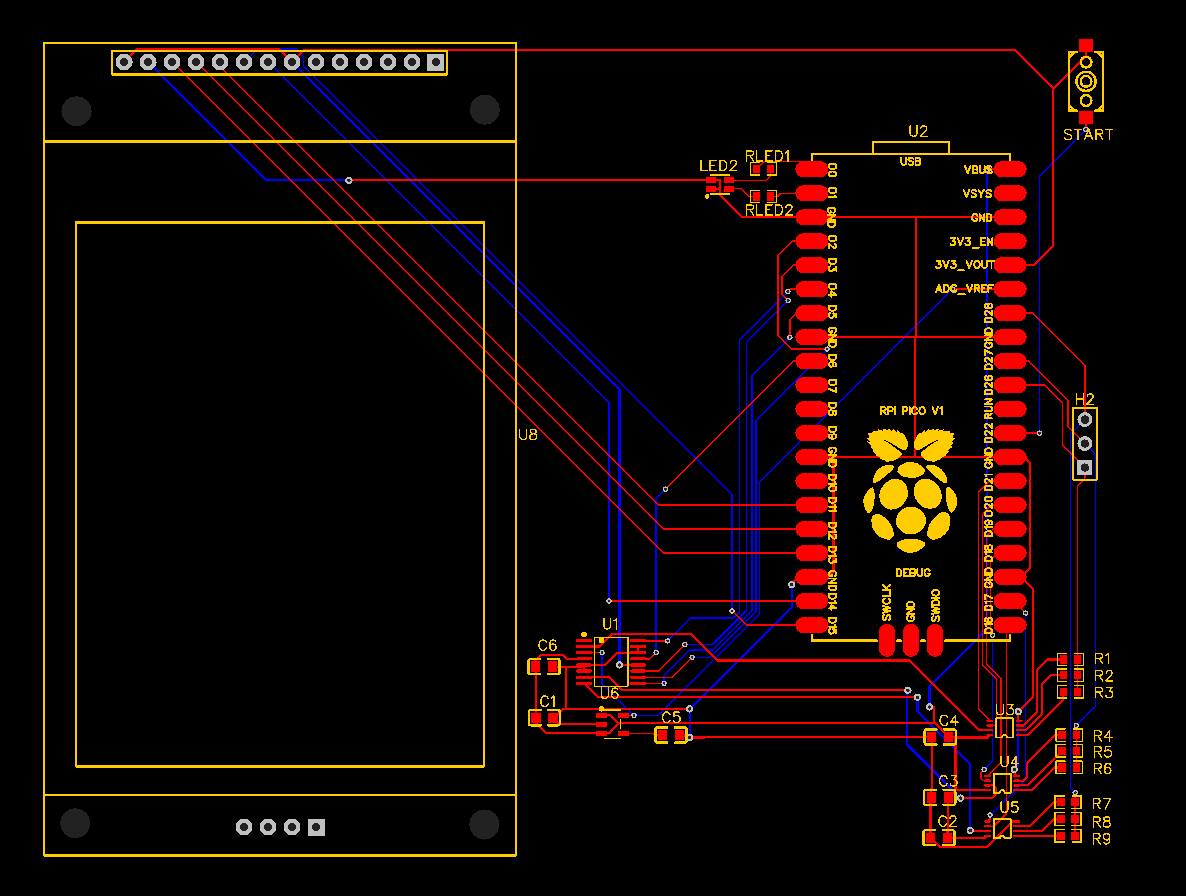
\includegraphics[scale=0.3]{images/literature/PCBV1.png}
    \caption{NYÁK első verziója}
    \label{fig:PCBV1}
\end{figure}

Legelső alkalommal a rendszer nem volt kivitelezhető, mivel túl vékony vezetékeket
használtam, ami nem volt legyártható a számomra elérhető helyeken. A komponenseket 
nehezen lehetett volna beilleszteni (Through Hole komponensek esetén, mint a kijelző),
mivel a vezetékek a lap mindkét oldalán voltak vezetve, így forrasztás során nehéz
lett volna azokat a lábakat forrasztani, amelyek a képernyő oldalán voltak.
Ezek át kellett vezessem olyan módon, hogy csakis a lap másik oldalán legyen a vezeték
csatlakoztatva a komponenshez.

Beszerzés során nem rendeltem meg minden alkatrészt, csak a fontosakat, így néhány
egyszerű alkatrészt helyettesítettem más alaktrésekkel, ez csupán egy feszültség referenciát
2 LED-et és egy kapcsolót érintett, így ezeket inkább helyileg helyettesítettem, minthogy
ismét rendeljem meg azokat.

A kijelző mérete a szerkesztőben és a valóságban nem egyezett meg, viszont ez még 
kiderült az áramkör kinyomtatása előtt, így nem vesztődött el sok idő. Az egész
kijelző nagyobb volt, mint a valóságban, még a láb közei is, így könnyedén látható
volt, hogy a tervrajz nem lesz kivitelezhető.

A tervrajzra nem tüntettem fel néhány jelzést, ami a felhasználást segíti, így ezt 
utólag felrajzoltam a lapra.

\subsection{Áramkör elkészítése}

Miután a tervezés elkészült és kivitelezhetőnek lett minősítve[\ref{fig:PCBV2}] azután az áramkör
el lett keszítve az egyetemi laboratórium segítségével. Miután a lapot a furatokkal és a réz
huzalozással megkaptam azután elkezdtem a komponensek felhelyezését.

\begin{figure}[h]
    \centering
    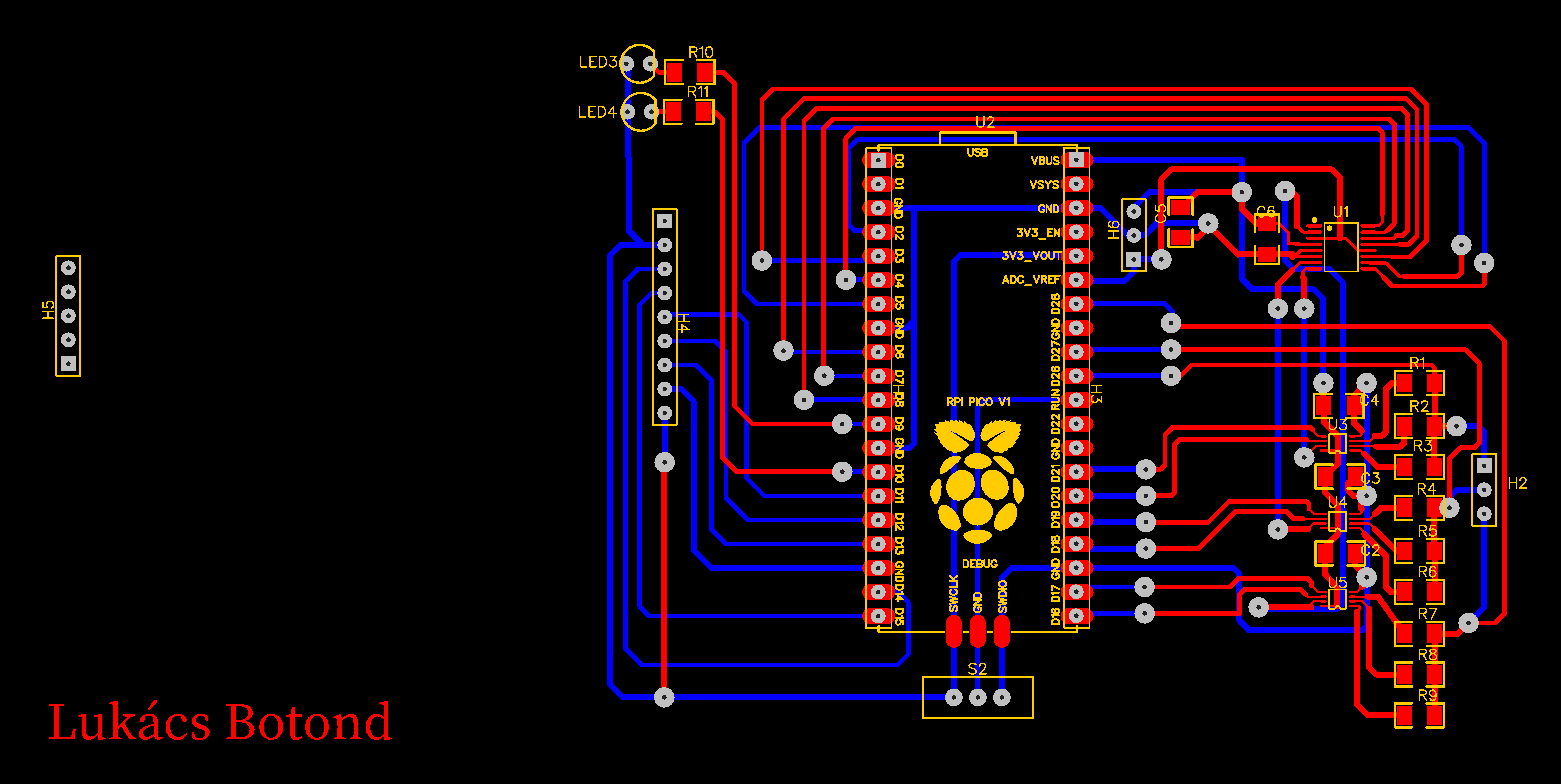
\includegraphics[scale=0.3]{images/literature/PCBV2.png}
    \caption{NYÁK végső verziója}
    \label{fig:PCBV2}
\end{figure}


Áramkör forrasztásával szintén nem volt sok tapasztalatom, csupán egyszerűbb
áramkörökkel, így nem a lehető legszebb, viszont használat során minden elektonikailag
csatlakoztatva van, így az áramkör működőképes. A végső áramkör a következőkben néz ki.
[\ref{fig:Aramkor}]


\begin{figure}[H]
    \centering
    \includegraphics[scale=0.1]{images/literature/PCB.jpg}
    \caption{A kész áramkör}
    \label{fig:Aramkor}
\end{figure}

\section{Szimulációk}

A szimulációra az LTspice \cite{LTspice} alkalmazást használtam, 
amelyben felépítettem a mérő áramkört és ellenőriztem, hogy az elméleti
mérési módszer alkalmas-e a mérés elvégzésére, és az értékek milyen
tartományban vannak, mivel a rendszer nem eléggé érzékeny, hogy a precíz
értékeket pontosan megadja, így olyan módszer kell ahol a tolerancia nagyobb.
Egy ilyen példa az áramerősség mérése amit a port ellenállást használja az
áramerősség meghatározására, viszont kis ellenállás esetén a
feszültség esés az ellenálláson alacsony áram esetén nem mérhető pontosan.
Ezért ilyen esetben nagyobb port ellenállást kell alkalmazni, hogy mérhető 
legyen a feszültség esés.

A program képes az időben változó feszültségeket is mérni, így
meg lehet tudni, hogy milyen idő intervalumban kell nézni és hogy
a komponensek időben mennyire befolyásolják a mérést. Ez 
legfőképpen a kondenzátorok mérésekor volt fontos, hogy megbizonyodjak
a mérések valóságosságáról.

A szimulációk többször is segítséget jelentettek a program 
hibáinak felfedezésében amit annélkül nehezebb lett volna felfedezni.



\chapter{Üzembe helyezés és kísérleti eredmények}
A teszter elkészítése után a rendszer tesztelése következett.
A rendszer nem fektetett nagy hangsúlyt a pontosságra, viszont egy 
megközelítő értéket meg kell tudjon határozni.

\section{Ellenállás mérés}

Amennyiben az elkatrész egy ellenállás akkor meghatározza ennek az ellenállását.
Mivel az ADC-n levő konstans és változó zajok vannak és ezen alapszik 
az áramerősség mérése, így a mérések pontossága nem magas[\ref{fig:ResistorResults}], ami különösen csökken a mérés tartomány
végén, mivel a mérő ellenállás amit az áramerősség mérésére használ túl alacsony így
nem képes pontosan meghatározni az áramerősséget. Ezt egy nagyobb mérő ellenállással
lehetne korrigálni.


\begin{table}[H]
    \begin{tabular}{|l|l|l|l|}
    \hline
    Sorszám & Névleges érték(Ohm) & Multiméterrel mért érték(Ohm) & Teszter által mért érték(Ohm) \\ \hline
    0       & 47             & 47                       & 52.5                     \\ \hline
    1       & 56             & 55.7                     & 59                       \\ \hline
    2       & 100            & 100.1                    & 107.4                    \\ \hline
    3       & 220            & 218                      & 242                      \\ \hline
    4       & 360            & 356                      & 398                      \\ \hline
    5       & 540            & 544                      & 606                      \\ \hline
    6       & 1000           & 980                      & 890                      \\ \hline
    7       & 2200           & 2198                     & 2301.7                   \\ \hline
    8       & 4700           & 4670                     & 4319.7                   \\ \hline
    9       & 10000          & 9680                     & 9237                     \\ \hline
    10      & 33000          & 32660                    & 28305.7                  \\ \hline
    11      & 62000          & 62000                    & 49590                    \\ \hline
    \end{tabular}
    \end{table}

    \begin{figure}[H]
        \centering
        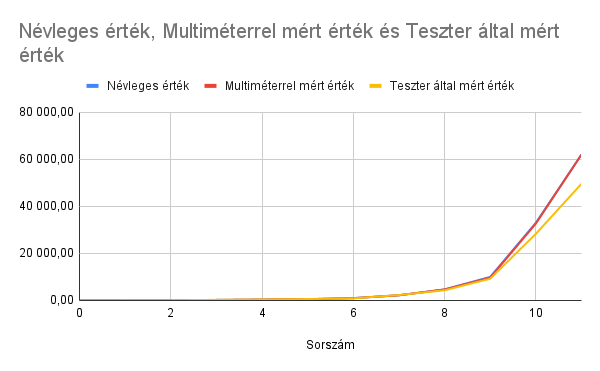
\includegraphics[scale=0.6]{images/results/resistorMesurement.png}
        \caption{Ellenállás mérés eredménye}
        \label{fig:ResistorResults}
    \end{figure}

    A tesztelés relatív hibája alább látható[\ref{fig:ResistorRelErrorResults}].
    \begin{figure}[H]
        \centering
        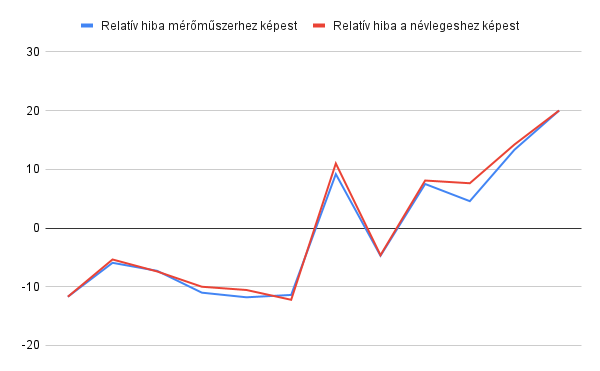
\includegraphics[scale=0.6]{images/results/RelErrorResistor.png}
        \caption{Ellenállás mérés relatív hibája}
        \label{fig:ResistorRelErrorResults}
    \end{figure}


\section{Kondenzátor}

Kondenzátor mérés estén az időt méri ameddig a kondenzátor feszültsége eléri a 
68\%-át a 3.3V-os forrásnak. Ezen esetben a mérés pontosabb, mivel
a zajok kevésbé befolyásolják így nem kell alacsony értékekből
számolni ami nagy hibához vezet. 50nF alatt nem biztos a mérés, 
mivel egyes alkatrészeket másnak is detektálhat, különösen ha 
hosszú vezetékek vannak használva. A grafikonon[\ref{fig:ResistorResults}]
látható, hogy a mérés jól megközelíti a névleges és dedikált mérőműszer
eredményeit.

\begin{table}[H]
    \begin{tabular}{|l|l|l|l|}
    \hline
    sorszám & Névleges érték & Mérőműszerrel mért érték & Mért érték \\ \hline
    1       & 60nF           & 59.62nF                  & 60nF       \\ \hline
    2       & 75nF           & 74.26                    & 75nF       \\ \hline
    3       & 100nF          & 98.26nF                  & 101nF      \\ \hline
    4       & 200nF          & 202nF                    & 203nF      \\ \hline
    5       & 300nF          & 300.3nF                  & 305nF      \\ \hline
    6       & 400nF          & 400nF                    & 406nF      \\ \hline
    7       & 500nF          & 498nF                    & 504nF      \\ \hline
    8       & 600nF          & 602nF                    & 610nF      \\ \hline
    9       & 700nF          & 701nF                    & 703nF      \\ \hline
    10      & 800nF          & 791.4nF                  & 800nF      \\ \hline
    11      & 900nF          & 889.7nF                  & 889nF      \\ \hline
    12      & 1uF            & 979nF                    & 1.059uF    \\ \hline
    13      & 2uF            & 1.97uF                   & 2.033uF    \\ \hline
    14      & 3uF            & 2.95uF                   & 3.05uF     \\ \hline
    15      & 4uF            & 3.96uF                   & 4.025uF    \\ \hline
    16      & 5uF            & 4.94uF                   & 5uF        \\ \hline
    17      & 6uF            & 5.935uF                  & 6.016uF    \\ \hline
    18      & 7uF            & 6.914uF                  & 6.95uF     \\ \hline
    19      & 8uF            & 7.946uF                  & 8.05uF     \\ \hline
    \end{tabular}
    \end{table}

    \begin{figure}[H]
        \centering
        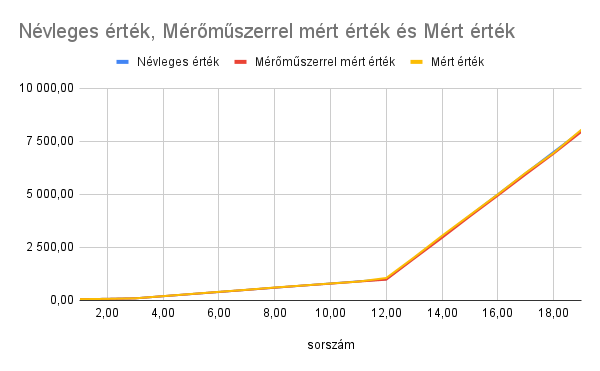
\includegraphics[scale=0.6]{images/results/CapacitorMeasurement.png}
        \caption{Kondenzátor mérés eredménye}
        \label{fig:CapacitorResults}
    \end{figure}

    A tesztelés relatív hibája alább látható[\ref{fig:CapRelErrorResults}].

    \begin{figure}[H]
        \centering
        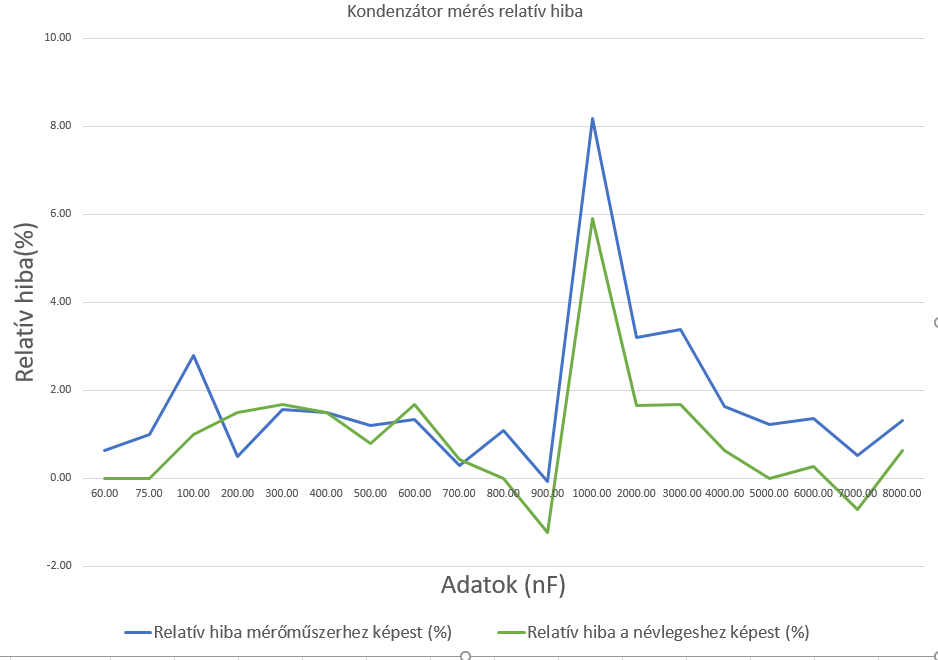
\includegraphics[scale=0.6]{images/results/CapRelError.png}
        \caption{Kondenzátor mérés relatív hibája}
        \label{fig:CapRelErrorResults}
    \end{figure}

\section{Dióda}

A dióda mérés a diódán eső feszültséget méri miközben az egyik oldala
tápfeszültségen van és a kapcsoló ellenállások használatával.
A mérések során azt tapasztaltam, hogy a multiméter alacsonyabb
értékeket adott, míg a teszter nagyobbakat, viszont a LED-ek
tesztelése során világosabban villant fel. Így arra a következtetésre
jutottam, hogy a multiméter azt a feszültséget mérte ahol
minimálisan elkezdett a dióda vezetni és a teszter meg amikor
már teljesen nyitva van. A kék LED esetében a multiméter nem volt képes
megmérni a nyitó feszültséget, viszont ez 2.5 és 3.7V közt helyezkedhet el.

2 inverz diódát is képes megmérni, ebben az esetben azt adja vissza, hogy melyik
irányban mekkora a dióda nyitó feszültsége.

\begin{table}[H]
    \begin{tabular}{lll}
    Sorszám                 & Mérőműszerrel mért érték                  & Mért érték                \\ \hline
    \multicolumn{1}{|l|}{0} & \multicolumn{1}{l|}{0,54}                 & \multicolumn{1}{l|}{0,69} \\ \hline
    \multicolumn{1}{|l|}{1} & \multicolumn{1}{l|}{1,58}                 & \multicolumn{1}{l|}{1,8}  \\ \hline
    \multicolumn{1}{|l|}{2} & \multicolumn{1}{l|}{1.85}                 & \multicolumn{1}{l|}{1,96} \\ \hline
    \multicolumn{1}{|l|}{3} & \multicolumn{1}{l|}{1,78}                 & \multicolumn{1}{l|}{2,01} \\ \hline
    \multicolumn{1}{|l|}{4} & \multicolumn{1}{l|}{kék LED, nem mérhető} & \multicolumn{1}{l|}{2,83} \\ \hline
\end{tabular}
\end{table}

\section{Tranzisztor}

Ebben az esetben a teszter megméri a tranzisztor lábkiosztását és az erősítését.
Képes az emitter és kollektor különbséget is meghatározni az erősítés nagyságából,
mivel az erősítés nagyobb abban az esetben, amikor a tranzisztor a helyes irányban
vezeti az áramot (NPN esetében az áram a kollektor emitter úton folyik).
Az erősítést akkor méri, amikor a tranzisztor kinyit, de még nincs teljesen kinyitva,
hanem a kollektor-emitter feszültség 2V körül van. Ezt a bázis feszültség
értékének a szabályozásával érhető el. Ekkor megméri a kollektor áramot
(mivel itt még nincs meghatározva, hogy melyik az, így most az ahonnan
az áram folyik) és elossza a bázison levő árammal.

Egy hiba a mérések alatt az volt, hogy a bázisra kis ellenállást
kapcsoltam és a tranzisztort a saturációs pontba tettem ahol 
nagy áram folyt a bázison keresztül ezért az erősítése nagyon alacsony
(5 alatt) volt, míg nagyobb ellenállással sem volt képes megközelíteni
az adatlapi értékét ebben az esetben. Amíg az új verzióval az 
erősítés sokkal jobban megközelíti a valóságot.

\section{Karakterisztika diagram}


\subsection{Kimeneti karakterisztika}

Az áramerősséget azon az értéken hagyva ahol a tranzisztor elkezdett kinyitni
végig mér a C-E feszültség 0-3.3V-os tartományán. A bázis használ egy 
P szabályozót, mivel a rendszer csak konstans feszültség forrást tartalmaz
és nem áramot. Az áram referencia ebben az esetben amikor a kollektor
emitter feszültsége eléri az 1.5V-ot

Minden mérési pontban megméri a kollektor
áramerősséget. Ezeket az eredményeket elmenti, majd kirajzolja a 
teszteren található kijelzőre. A kirajzolás csak a kijelzőn
jelenik meg, mivel egy egyszerű Serial port olvasó program
szöveg megjelenítésére használatos és nincs számítógép oldani applikáció.

A PNP tranzisztor esetében az emitter konstans 3.3V-on tartásával és 
kollektor csökkentésével 3.3V-ról a emitter-kollektor feszültség
0 és 3.3V közt változik, miközben a bázis feszültsége sosem negatív
a földhöz képest.

A mérés a következőképpen lesz látható a kijelzőn[\ref{fig:OutChar}] 

\begin{figure}[H]
    \centering
    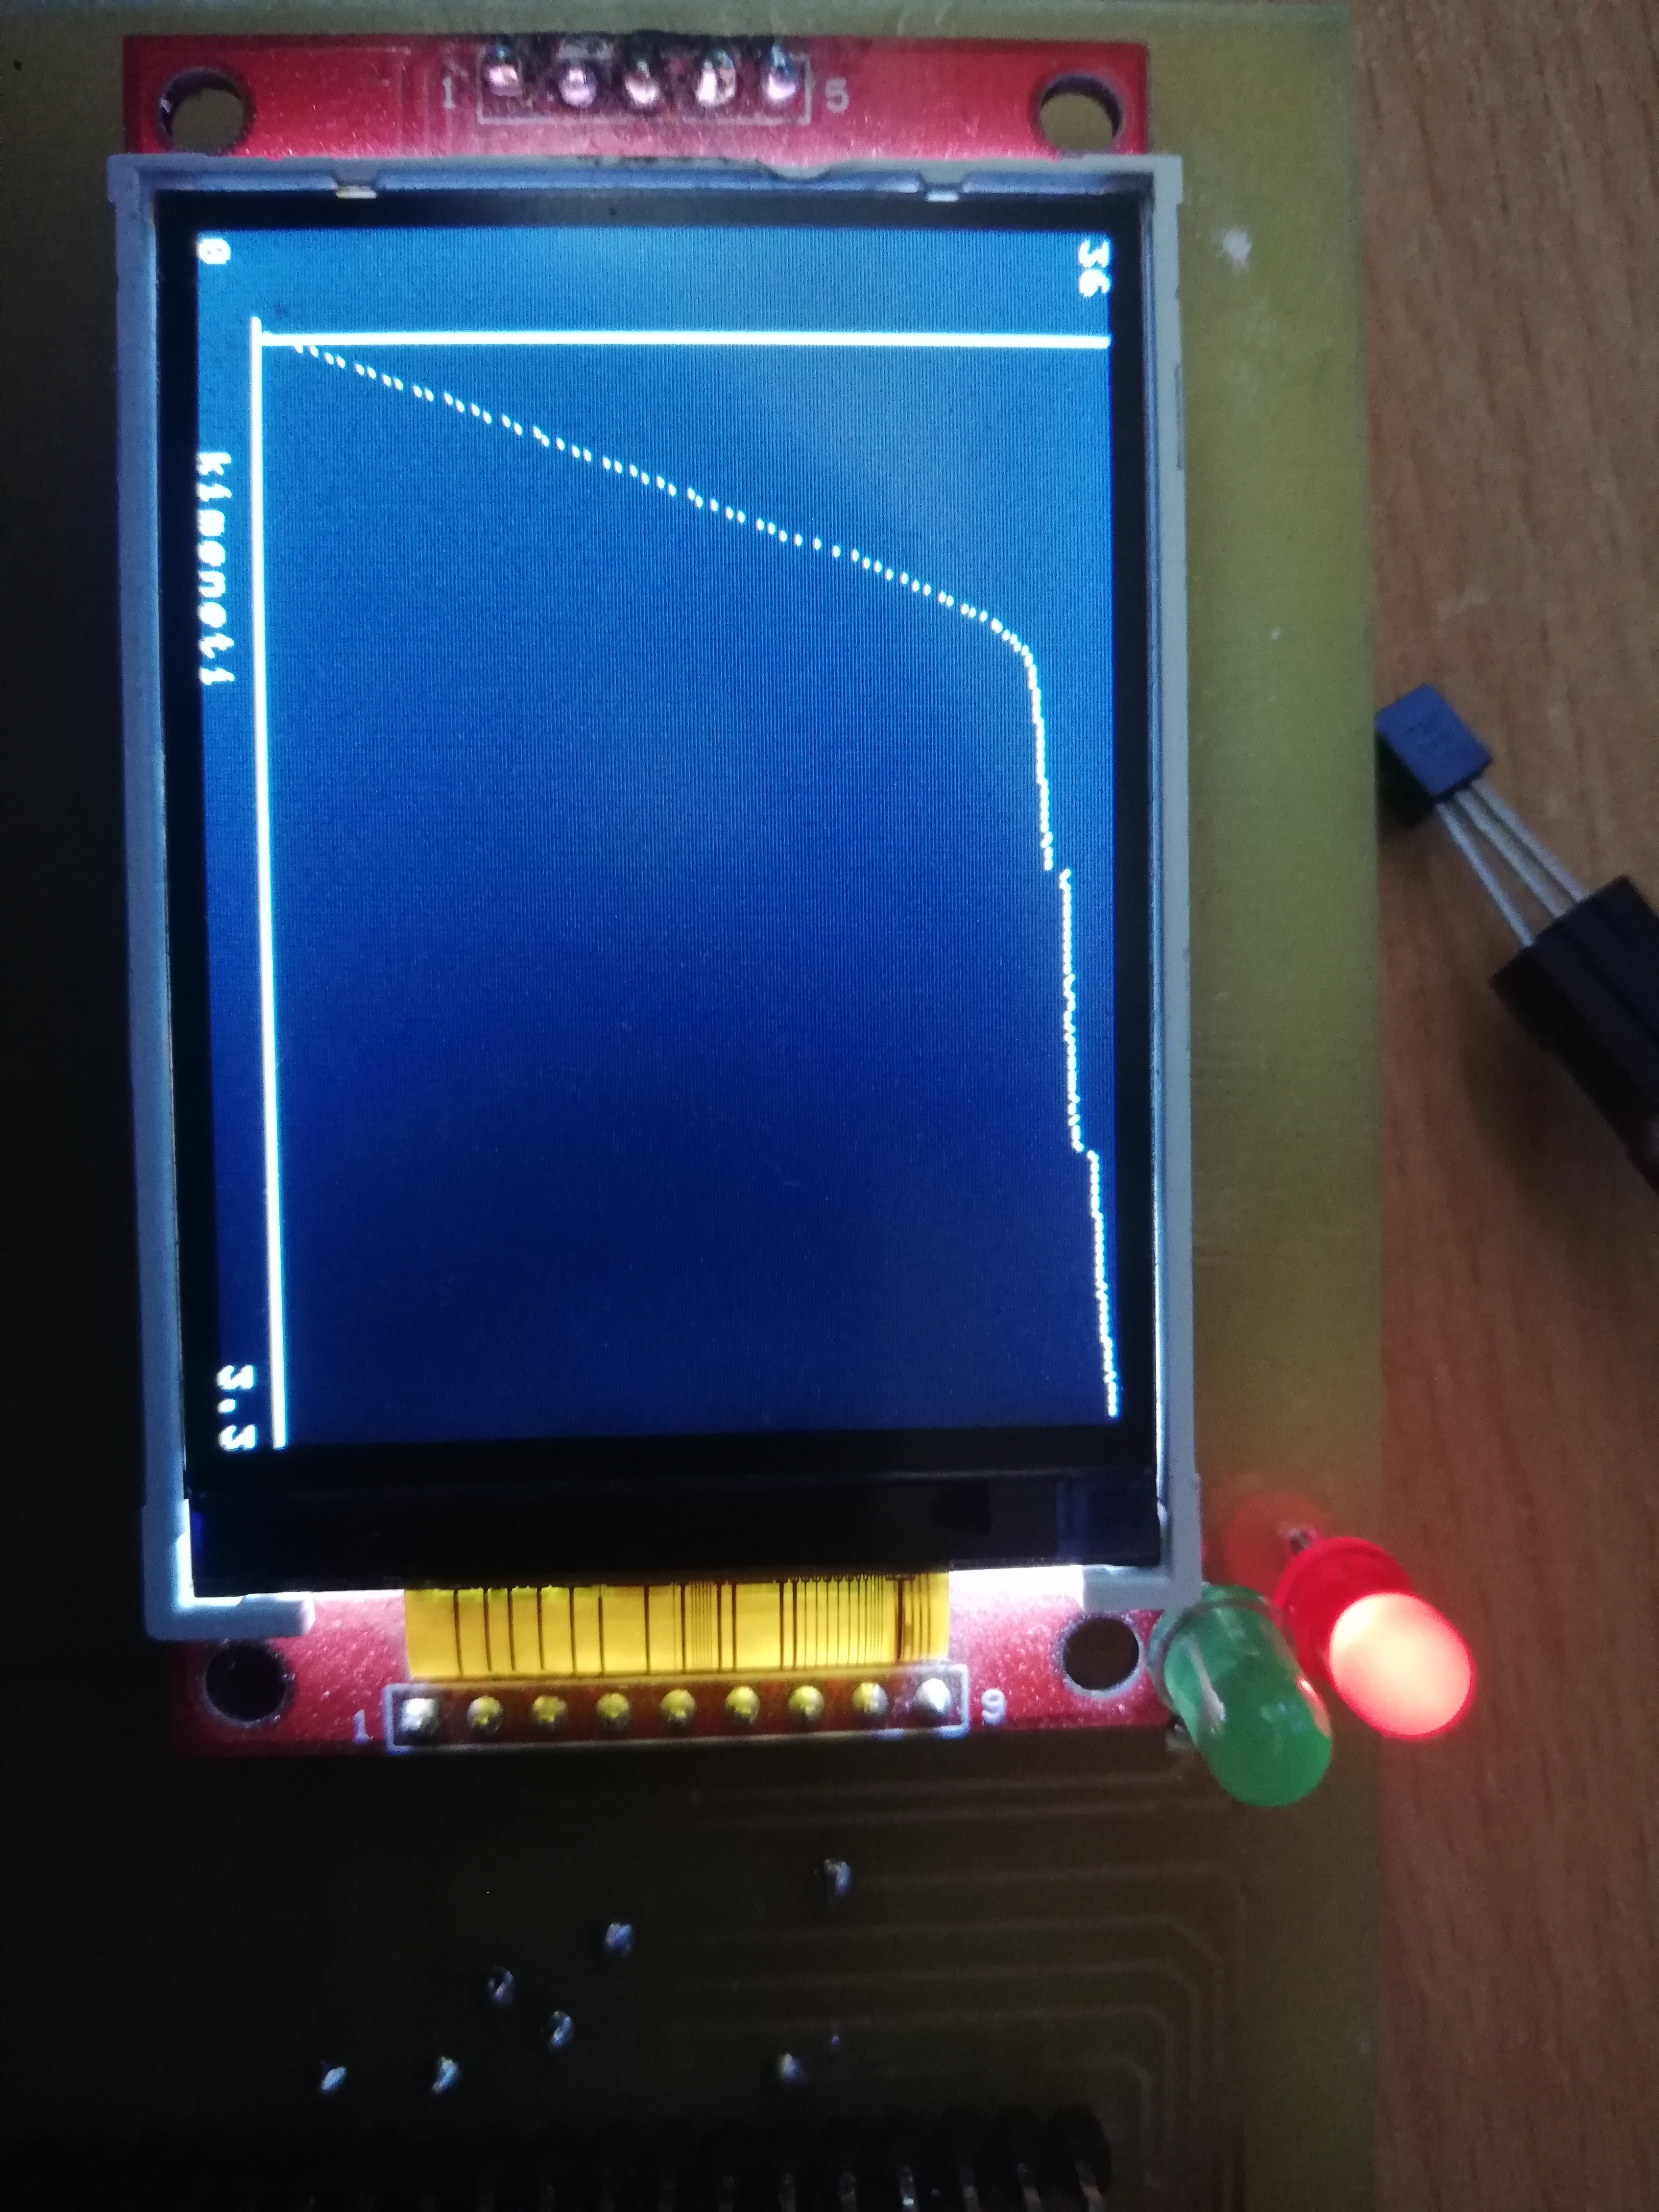
\includegraphics[scale=0.1, angle=90]{images/results/OutChar.jpg}
    \caption{Kimeneti karakterisztika diagram}
    \label{fig:OutChar}
\end{figure}

\subsection{bemeneti karakterisztika}

Ebben az esetben a kollektor és az emitter a földre van kötve,
miközben a bázis feszültség növekedik. A kapcsoló ellenálláson eső feszültségből
kiszámítható az áram. A diagram a dióda karakterisztikához hasonló eredményt
ad.[\ref{fig:InChar}] 

\begin{figure}[H]
    \centering
    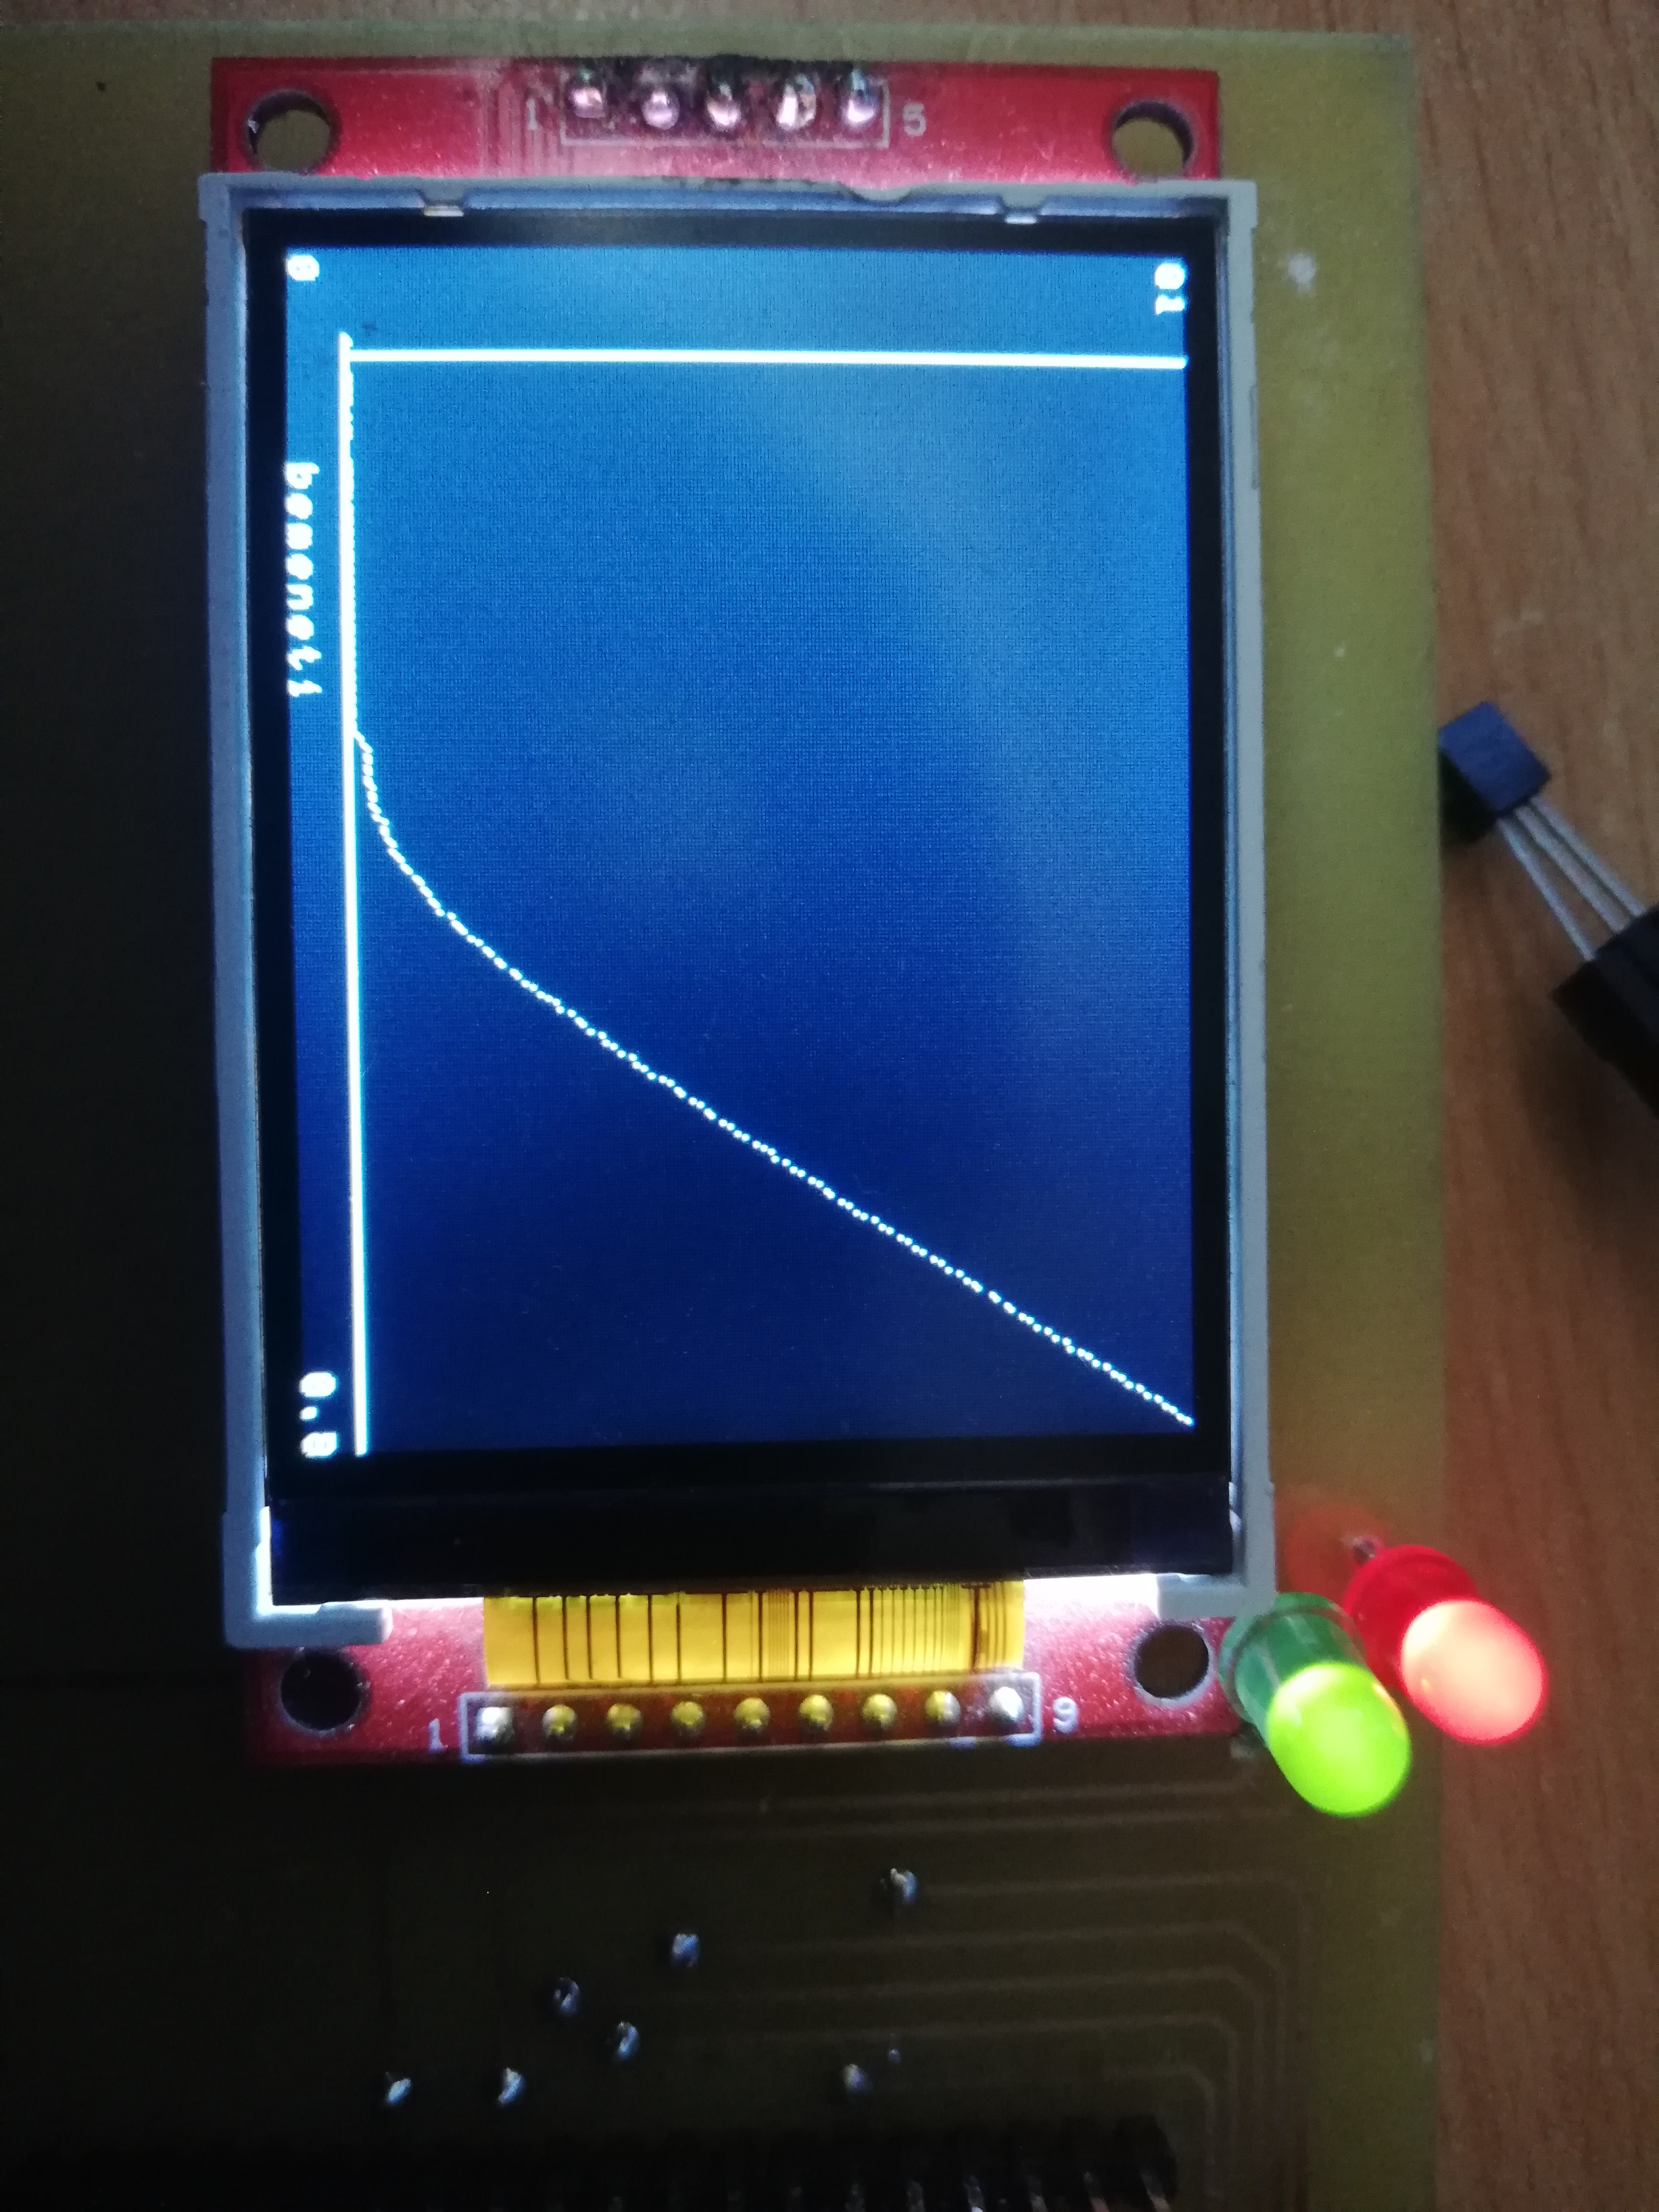
\includegraphics[scale=0.1, angle=90]{images/results/InChar.jpg}
    \caption{Bemeneti karakterisztika diagram}
    \label{fig:InChar}
\end{figure}



\chapter{A rendszer felhasználása}
\input{chapters/rendszerFelhasznalasa}

%következtetés
\chapter{Következtetések}
\section{Megvalósítások}

A projekten belül egy olyan rendszer megvalósítására került sor,
amellyel leegyszerűsíthetőek az alkatrészek azonosítása és mérése.
A megvalósítás során sikerült az egyszerű alkatrészek azonosítása
és mérése, miközben megközelítőleg az értékei is meghatározására
kerültek.

A megvalósítás során fő szempont volt az egyszerűség a felhasználó felé,
így nem kell tudjon semmit az eszközről és elvégezni komplex műveleteket,
hogy az eredményt megkapja. 


\section{Hasonló rendszerrel való összehasonlítás}

A hasonló rendszer ami alapján terveztem a rendszert \cite{similarSystem}
több dolog detektálására is képes, viszont az egy nyílt forráskódú
projekt, amit többen is tovább fejlesztettek az idők során. Viszont
ebből csak részben a mérő áramkör ami hasonló, pontosabban ellenállások
használata változtatható feszültség forrásra van kapcsolva. 
Ebben az esetben viszont csak digitális feszültség szinteket lehet
használni, mivel az a rendszer nem alkalmaz egy DAC-ot.

Mindkét rendszer képes kiírni egy kijelzőre ami a teszteren található
a mérések eredményeit. Viszont a hasonló eszköz nemcsak a lábkiosztását,
hanem az áramköri rajzát is megjeleníti.

Viszont a hasonló eszköz nem képes változtatható feszültséggel vezérelni a
komponenst, így nem képes karakterisztika diagramok kirajzolására.

\section{További fejleszési lehetőségek}

A rendszernek lehetősége volna komplexebb alkatrészek
tesztelésére is, viszont a 3.3V-os feszültség határ
korlátoz sok esetben is. Például a MOSFET-ek tesztelése nagyobb
feszültségre lenne szükség, hogy biztosan azonosíthatóak legyenek.
Ezen kívül többféle dióda és tranzisztor fajták vannak, 
amelyekre komplexebb azonosítási algoritmus szükséges.

A rendszerrel lehetséges lenne állítható frekvenciával tekercsek mérésére
is és különböző típusú jelek generálása.

Módosítás az áramkörön, hogy a teszter socket biztosabb legyen, mivel
jelenleg egyes esetekben nem érintkezhet megfelelően ezért hibás az azonosítás.

Az áramkör módosítása olyan módon, hogy lehetséges legyen SMD alkatrészeket
is könnyedén tesztelni.

A mérési tartomány kiterjesztése a mérő ellenállások cseréjével.





%irodalomjegyzek
\addcontentsline{toc}{chapter}{Irodalomjegyzék}

\bibliographystyle{ieeetr}
\bibliography{References}

%appendix
\appendix
\chapter{Függelék}
\input{chapters/fuggelek}



\end{document}
